\documentclass[journal]{IEEEtran}

% , - Packages , , , , , , , , , , , , , , , , , , , -
\usepackage[utf8]{inputenc}
\usepackage[T1]{fontenc}
\usepackage{textcomp}
\usepackage{amsmath,amssymb,amsfonts}
\usepackage{graphicx}
\usepackage{subfig}
\usepackage{bm}
\usepackage{url}
\usepackage{xcolor}
\usepackage[colorlinks=true,allcolors=blue]{hyperref}

% , - Convenience macros , , , , , , , , , , , , , , , , -
\newcommand{\Tris}{T-RIS}
\newcommand{\Rris}{R-RIS}
\DeclareMathOperator*{\argmax}{arg\,max}

\graphicspath{{figures/}}
\begin{document}

\title{A Two-Stage Reconfigurable Intelligent Surface\\
Architecture for Decoupled M-FSK Modulation and\\
Beamforming in 28-GHz Bistatic Sensing}

\author{Jaswinder Lota,~\IEEEmembership{Senior Member,~IEEE,}
        Pavan Mohan Neelamraju,~\IEEEmembership{Student Member,~IEEE,}
        William Whittow,~\IEEEmembership{Senior Member,~IEEE,}
        Andreas Demosthenous,~\IEEEmembership{Fellow,~IEEE,}
        and Aakash Bansal,~\IEEEmembership{Member,~IEEE}

\thanks{This work was supported by the UKRI Engineering and Physical Sciences Research Council through the A-PLUS Project under Grant UKRI3212.}

\thanks{J. Lota is with the Department of Engineering and Construction, University of East London, University Way, London E16 2RD, U.K.}

\thanks{P. M. Neelamraju, W. Whittow, and A. Bansal are with the Wolfson School of Mechanical, Electrical and Manufacturing Engineering, Loughborough University, Loughborough LE11 3TU, U.K.}

\thanks{A. Demosthenous is with the Department of Electronic and Electrical Engineering, University College London, London WC1E 7JE, U.K.}

\thanks{Corresponding author: Pavan Mohan Neelamraju (e-mail: npavanmohan3@gmail.com).}
}

\markboth{IEEE Transactions on Vehicular Technology,~Vol.~XX, No.~X, Month~Year}%
{Author \MakeLowercase{\textit{et al.}}: A Two-Stage RIS Architecture for Decoupled M-FSK Modulation and Beamforming}

\maketitle

\begin{abstract}
This paper presents a two-stage reconfigurable intelligent surface (RIS) that synthesizes a multiple-frequency-shift-keying (M-FSK) sensing waveform at 28\,GHz. A transmissive RIS (T-RIS), driven by a single direct digital synthesizer (DDS), modulates a continuous-wave carrier into stepped tones, and a reflective RIS (R-RIS) beamforms all tones toward the target. The separation confines radio-frequency switching to the T-RIS, so the R-RIS is updated once per coherent processing interval (CPI) and can use slow, high-resolution devices. We derive the bistatic link budget and Cram\'{e}r--Rao bounds (CRBs) for path, velocity, angle and position, and show that a coherent two-dimensional estimator with peak refinement attains them, with 1.84\,cm path and 2.45\,cm position root-mean-square error (RMSE) at a $60^\circ$ bistatic angle. The tones are separated in a complex-baseband receiver without a high-$Q$ filter, their beam squint costs 0.03\,dB, and element phase noise of $27^\circ$ costs 1\,dB without degrading estimator efficiency. A Rayleigh--Sommerfeld analysis of the inter-stage coupling gives assembly tolerances of 0.70\,mm in gap and 1.86\,mm laterally. An interacting multiple-model tracker that fuses the Doppler measurement keeps the position RMSE between 0.9 and 1.5\,cm for straight, accelerating and turning trajectories. With identical accounting, the transmit side draws 25\,\% less power than a 5-mW-per-channel CMOS active electronically scanned array, breaking even at 2.7\,mW per channel, and at equal CPI the waveform matches chirp-sequence frequency-modulated continuous-wave radar in multi-target resolution.
\end{abstract}

\begin{IEEEkeywords}
Bistatic Radar, Cram\'{e}r-Rao bound, beamforming, integrated sensing and communication, M-ary frequency-shift keying, millimeter-wave sensing, Reconfigurable intelligent surface, space-time modulation.
\end{IEEEkeywords}

\section{Introduction}
\IEEEPARstart{R}{econfigurable} intelligent surfaces (RIS) have emerged as a
key enabler for beyond-5G wireless systems, offering electronically
controlled spatial beamforming at low hardware cost and without active RF
chains~\cite{wu2019towards,basar2019wireless}. A RIS comprises a planar
array of sub-wavelength elements whose reflection or transmission phase is
tunable via PIN diodes, varactor diodes, or MEMS switches. The conventional
role of a RIS is purely passive: it redirects an impinging wave toward a
target direction by applying a spatial phase gradient across the
aperture~\cite{hu2018beyond,marzetta2015massive,liaskos2018new,wu2019intelligent}.
However, if the element impedances are modulated at a frequency $f_m$ by a
time-varying control signal, the transmitted or reflected field acquires
frequency-shifted components at $f_c \pm f_m$ alongside the original carrier
at $f_c$. This space-time-modulated (STM) RIS concept~\cite{zhang2018space}
elevates the RIS from a passive reflector to an active waveform system,
replacing the complex and power-hungry RF transmitter (Tx) chains with a
single continuous-wave (CW) source.

M-ary frequency-shift keying (M-FSK) is a widely deployed radar waveform
for the joint estimation of target range and velocity. Unlike binary FSK,
which resolves velocity alone, or pulsed radar, which is optimized for
range, an M-FSK radar combines discrete frequency steps with coherent
processing to resolve both range and velocity within a single coherent
processing interval (CPI), with negligible range--Doppler coupling and with the capability to discriminate multiple targets
simultaneously~\cite{rohling2001waveform}. Recent work emphasizes the
robustness of M-FSK in strong-multipath environments, indoor sensing and
dense urban automotive scenarios and its suitability for integrated
sensing and communication ~\cite{lu2024integrated}. Generating M-FSK
directly from an STM-RIS, by programming the modulation frequency $f_m$ to
one of $M$ offset values per symbol, promises a markedly simpler
millimeter-wave (mmWave) front-end that dispenses with the IQ modulator and
mixer chain. The design challenge addressed here is that such an approach
must simultaneously (i) synthesize the desired upper sideband at
$f_c + f_m$, (ii) steer the radiated beam to a specified azimuth and
(iii) reject the image sideband at $f_c - f_m$ that unavoidably accompanies
the impedance modulation.

\subsection{The Single-Stage Bottleneck}
Existing STM-RIS work has demonstrated that a single surface can, in
principle, perform modulation and beamforming
simultaneously~\cite{zhang2018space,zhang2019breaking,dai2018independent}.
The theoretical foundation is the space-time-coding digital metasurface
framework~\cite{zhang2018space}, where each element is assigned a
temporal switching sequence. By jointly designing the harmonic content and
the spatial phase gradient of these sequences, the surface translates
frequency and steers the resulting beam to a programmed direction. For
M-FSK, a single STM-RIS would assign each element $n$ a Direct-Digital Synthesizer (DDS)-driven bias
signal with a phase offset corresponding to the desired beam direction,
producing an upper sideband at $f_c + f_m$ steered to $+\theta$ and an image
at $f_c - f_m$ steered to $-\theta$. A related hardware demonstration
implements simultaneous beam steering and on-off-keying (OOK) amplitude
modulation at 100\,GHz using a transmissive Pancharatnam-Berry phase RIS
with Schottky-diode elements~\cite{shen2025sub}, exploiting
the orthogonality between the spatial coding sequence (which sets beam
direction) and the temporal switching sequence (which sets the OOK data).

While chirped Frequency-Modulated Continuous Wave (FMCW) waveforms remain standard in macro-scale, high-velocity automotive environments, the orthogonal parameter isolation of M-FSK presents an exceptional candidate for energy-constrained micro-mobility platforms, automated guided vehicles in smart industrial logistics and localized robotic drone tracking where range-Doppler cross-term coupling must be completely eliminated without complex multi-slope active RF transceiver architectures.

However, the single-stage approach faces a fundamental limitation when
applied to M-FSK. In OOK the beam direction is fixed and only the symbol
amplitude changes; in M-FSK the symbol frequency $f_m$ changes at every symbol
period, requiring every element's modulation to carry its beamforming phase. If the phase maps are reloaded over a 10\,MHz serial peripheral interface (SPI), 256 elements at 3 bits take 76.8\,$\mu$s per symbol, which limits the symbol rate to 13\,kHz. Look-up tables and field-programmable gate array (FPGA) parallel loading remove this control bottleneck~\cite{zhang2018space,zhao2019programmable,liaskos2022software}; 16 parallel chains at 100\,MHz reload the map in 0.48\,$\mu$s. What remains is physical: a single surface that both modulates and beamforms must switch every beamforming element at the modulation rate, either with element-specific phase offsets, whose time-coded implementation requires a timing resolution of $1/(2^B f_{m,M}) = 0.42$\,ns, or with a global 0/$\pi$ line that toggles every element's phase state. In either case the beamforming elements must be fast-switching devices.
 Moreover, the single-stage design steers the
image sideband to $-\theta$, providing only $\sim$13\,dB of image rejection
set by the array-factor sidelobe level of a uniformly weighted 16-element
aperture; adequate rejection would otherwise demand a tapered aperture
(sacrificing directivity) or a post-detection spatial filter.

\subsection{Contributions}
This paper proposes a two-stage RIS architecture that decouples modulation
from beamforming, attaining full DDS-limited symbol rates with an
independently steerable beam. In the first stage, the \Tris{} elements are
driven identically by a single DDS with no spatial phase; new
M-FSK symbol is selected by writing a new tuning word to one DDS
register, requiring no per-element SPI update. The output is a
dual-sideband field at $f_c \pm f_m$ with uniform spatial weighting. In the
second stage, the \Rris{} applies the beamforming phase gradient $\psi_n$
independently of the symbol being transmitted: the beam angle is set once
at acquisition and updated only when the target direction changes, not per
symbol. Because the \Rris{} co-steers the image with the desired sideband, the two are separated in the complex-baseband (I/Q) receiver, where they occupy opposite halves of the spectrum; no high-$Q$ radio-frequency filter is required (Section~\ref{sec:sideband}).
Concretely, the contributions are:
\begin{enumerate}
\item A physically separated two-stage \Tris/\Rris{} architecture that confines radio-frequency switching to one layer driven by a single DDS, so that the beamforming layer is updated once per CPI and can use slow, high-resolution devices;
\item A closed-form bistatic link budget that explicitly accounts for
near-field inter-stage evanescent coupling, together with CRBs for range,
velocity and 2-D position, a coherent estimator that attains them and an attribution of every source of estimation error;
\item A closed-loop IMM beam-tracking loop with Doppler fusion, validated for straight, accelerating and turning trajectories; and
\item A system-level study of power consumption, multi-target capability,
and inter-stage assembly and phase-noise tolerances, and receive-aperture scaling quantifying the practicality of the architecture for energy-constrained mmWave platforms.
\end{enumerate}
The remainder of the paper is organized as follows. Section~\ref{sec:model}
develops the modulation and beamforming model and the bistatic signal
model. Section~\ref{sec:tracking} presents the estimators, their CRBs and
the tracking loop. Section~\ref{sec:results} reports the device, waveform,
sensing and tracking results. Section~\ref{sec:design} analyzes
multi-target capability, system power and gap sensitivity.
Section~\ref{sec:conclusion} provides concluding remarks.

\section{RIS M-FSK Modulation}
\label{sec:model}

\begin{figure}[!t]
\centering
\subfloat[Bistatic geometry (Table~\ref{tab:sys_params})]{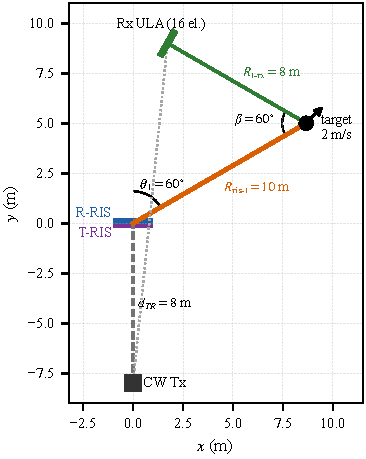
\includegraphics[width=0.95\columnwidth]{F1a_scene}\label{fig:overview_a}}
\\ \vspace{0.5em}
\subfloat[Signal and control flow]{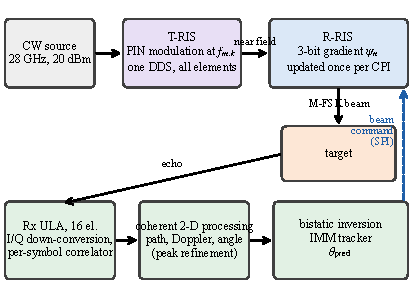
\includegraphics[width=0.95\columnwidth]{F1b_process_flow}\label{fig:overview_b}}
\caption{Overview of the two-stage \Tris/\Rris{} M-FSK bistatic sensing
system at 28\,GHz. A CW transmitter illuminates the transmissive \Tris,
which generates the M-FSK sidebands; the reflective \Rris{} applies the
beamforming phase gradient and steers all tones toward the target. The
scattered field is collected by a bistatic receive array.}
\label{fig:overview}
\end{figure}

\subsection{System Overview}
The proposed system comprises a CW Tx, a two-stage stacked RIS employing PIN
diodes and a bistatic receiver (Rx), as illustrated in
Fig.~\ref{fig:overview}. The Tx radiates a CW signal at $f_c$ and is located
at distance $d_{TR}$ from the RIS stack. Each RIS stage is a planar aperture
of $N$ elements with half-wavelength spacing. The target lies at azimuth
$\theta_1$ from the RIS, while the Rx is at azimuth $\theta_2$; the two
stages are separated by an inter-stage gap $d_g$. Stage one is a
transmissive (\Tris) surface and stage two is a passive reflective (\Rris)
surface with $B$-bit phase quantization per element.

The \Tris{} element is modeled using an experimentally validated equivalent
lumped circuit~\cite{demmer2023hybrid}, scaled to 28\,GHz PIN-diode
parameters~\cite{dai2020reconfigurable}. Each transmissive element presents
a series-connected diode impedance $Z_1(f,\mathrm{state})$ in a feed-line
environment of characteristic impedance $Z_0 = 50\,\Omega$. The diode
equivalent circuit consists of a series resistance $R_s$ (bond-wire and
contact parasitics) in series with the parallel combination of a
state-dependent junction resistance $R_J(\mathrm{state})$ and the junction
capacitance $C_J$:
\begin{equation}
Z_1(f,\mathrm{state}) = R_s + \frac{R_J(\mathrm{state})}
{1 + j\omega C_J R_J(\mathrm{state})},
\label{eq:diode_Z}
\end{equation}
where $\omega = 2\pi f$. The adopted 28-GHz parameters are
$R_s = 2\,\Omega$, $C_J = 25$\,fF, $R_J(\mathrm{on}) = 1\,\Omega$ and
$R_J(\mathrm{off}) = 8\,$k$\Omega$~\cite{pozar2011microwave,dai2020reconfigurable}.
Modeling the element as a series impedance in a matched $Z_0$ line, the
transmission coefficient is~\cite{dai2020reconfigurable}
\begin{equation}
T_n(f,\mathrm{state}) = \frac{2Z_0}{2Z_0 + Z_1(f,\mathrm{state})}.
\label{eq:Tn}
\end{equation}
Evaluating \eqref{eq:Tn} at $f_c = 28$\,GHz yields $T_n(f,\mathrm{on})$ and
$T_n(f,\mathrm{off})$ separated by a phase difference of $64.5^\circ$. The
phase asymmetry arises because in the on-state $C_J$ is effectively
short-circuited, whereas in the off-state $C_J$ introduces a significant
reactive component.

The proposed M-FSK waveform uses $M = 12$ tone frequencies, all placed on
the upper (positive) sideband of the carrier. Denoting the symbol index
$k \in \{1,\dots,M\}$, the frequency offset of symbol $k$ is
\begin{equation}
f_{m,k} = k\,\Delta f,
\label{eq:fmk}
\end{equation}
yielding tones at $\{25, 50, \dots, 300\}$\,MHz above $f_c$. Placing all desired tones on one sideband ensures that, after down-conversion with the local oscillator at $f_c$, every desired tone occupies the positive half of the complex-baseband spectrum and every image the negative half; bidirectional offsets would place the images of positive-offset tones on top of negative-offset tones. The separation is performed digitally (Section~\ref{sec:sideband}).
 The \Tris{}
elements are driven identically by a single DDS with $\varphi_n = 0$ for all
$n$. Modeling the PIN diode as a switch driven between its on- and off-states
by the DDS sinusoid at frequency $f_m$, the instantaneous transmission
coefficient of element $n$ is~\cite{zhao2019programmable,song2018beam}
\begin{align}
T_n(t,f) ={}& T_{\mathrm{mean}}(f) \nonumber\\
&+ \frac{T_n(f,\mathrm{on}) - T_n(f,\mathrm{off})}{2}\cos\!\left(2\pi f_m t + \varphi_n\right),
\label{eq:Tnt}
\end{align}
where
\begin{equation}
T_{\mathrm{mean}}(f) = \frac{T_n(f,\mathrm{on}) + T_n(f,\mathrm{off})}{2}
\label{eq:Tmean}
\end{equation}
is the quiescent transmission and the second term is the sinusoidal
modulation about that bias point. Multiplying \eqref{eq:Tnt} by the incident
CW carrier constitutes a resistive mixing process~\cite{zhao2019programmable},
producing the transmitted signal at element $n$,
\begin{equation}
s_n(t) = T_n(t,f)\cos(2\pi f_c t).
\label{eq:sn}
\end{equation}
Applying the product-to-sum identity with $\varphi_n = 0$ to
\eqref{eq:Tnt}-\eqref{eq:sn} gives
\begin{align}
s_n(t) ={}& T_{\mathrm{mean}}(f)\cos(2\pi f_c t) \nonumber\\
&+ \frac{T_n(f,\mathrm{on}) - T_n(f,\mathrm{off})}{4}
\big[\cos(2\pi (f_c + f_{m,k})t) \nonumber\\
&\quad + \cos(2\pi (f_c - f_{m,k})t)\big].
\label{eq:sn_expand}
\end{align}
Each element output thus contains three spectral components: a residual
carrier at $f_c$ of amplitude $T_{\mathrm{mean}}(f)$, the desired upper
sideband at $f_c + f_{m,k}$ and the image at $f_c - f_{m,k}$. Both sidebands
have equal amplitude, half the modulation depth,
\begin{equation}
T_{\mathrm{sb}}(f) = \frac{T_n(f,\mathrm{on}) - T_n(f,\mathrm{off})}{2}.
\label{eq:Tsb}
\end{equation}

\subsection{R-RIS Beamforming and Near-Field Coupling}
In stage two the \Rris{} applies a spatial phase gradient to steer the
combined radiated field toward the target at azimuth $\theta_1$. The
per-element reflection phase is
\begin{equation}
\psi_n = k_c\, x_n \sin\theta_1,
\label{eq:psi}
\end{equation}
where $k_c = 2\pi f_c / c$ is the free-space wavenumber and $x_n$ is the
$x$-coordinate of element $n$. Each \Rris{} element is a PIN-diode reflector
with complex reflection coefficient~\cite{dai2020reconfigurable}
\begin{equation}
\Gamma = |\Gamma|\,e^{j\psi_n},
\label{eq:Gamma}
\end{equation}
where $|\Gamma| \approx 0.89$ ($-1$\,dB). Because $\psi_n$ is computed at the
carrier wavenumber $k_c$ and is independent of the symbol index $k$, the
\Rris{} is programmed once at acquisition and requires no per-symbol update.
This independence of beam direction from symbol frequency is the structural
advantage of the two-stage architecture over single-surface STM-RIS
designs~\cite{zhang2018space}, in which changing the symbol frequency
would mandate reprogramming all element phases.

Because the two stages are separated by only $\approx 0.19\lambda$, the
\Rris{} lies within the near-field of the \Tris. The field coupling from a
\Tris{} element to the co-located \Rris{} element is~\cite{marcuvitz1951waveguide,pfeiffer2013cascaded}
\begin{equation}
C_0 = e^{-\alpha(f)\, d_g},
\label{eq:C0}
\end{equation}
where $d_g$ is the nominal inter-stage gap and $\alpha(f) = 2\pi/\lambda$ is
the evanescent near-field decay constant. The field at each \Rris{} element
is the superposition of contributions from all \Tris{} elements; the
dominant term is the co-located element, while off-axis contributions carry
rapidly varying propagation phases that interfere destructively, leaving a
net coupled amplitude $\approx C_0$~\cite{monticone2017metamaterial}. This is the
on-axis near-field approximation of the Rayleigh-Sommerfeld inter-layer
propagation model used in the stacked-intelligent-metasurface (SIM)
designs ~\cite{an2025stacked}. Unlike SIM architectures, where $d_g$ is
deliberately tuned to realize a prescribed inter-layer coupling matrix for
holographic beamforming, here $d_g$ is an unavoidable mechanical-assembly loss, with $C_0^2$ entering the link budget \eqref{eq:Prx} as a power penalty. Equation~\eqref{eq:C0} retains only the co-located term. Section~\ref{sec:5b} evaluates the full Rayleigh--Sommerfeld model by angular-spectrum propagation between the two finite apertures: for element apertures filling half of the cell width it gives $-11.1$\,dB at $d_g = 2$\,mm, within 0.9\,dB of \eqref{eq:C0}, but it saturates beyond $d_g \approx 3$\,mm, because the fundamental Floquet mode propagates without decay. Equation~\eqref{eq:C0} is therefore valid only near the nominal gap and overstates the gap sensitivity. The link budget of Section~\ref{sec:linkbudget} uses the full-model value.

\begin{table}[!t]
\renewcommand{\arraystretch}{1.15}
\caption{System Parameters}
\label{tab:sys_params}
\centering
\begin{tabular}{l l r}
\hline\hline
Parameter & Symbol & Value \\
\hline
Carrier frequency & $f_c$ & 28 GHz \\
Free-space wavelength & $\lambda$ & 10.71 mm \\
Tx radiated power & $P_{\rm Tx}$ & 20 dBm (0.1 W) \\
Tx antenna gain & $G_{\rm Tx}$ & 0 dBi \\
Target RCS & $\sigma_{\mathrm{RCS}}$ & 0 dBsm (1 m\textsuperscript{2}) \\
Tx-RIS distance & $d_{TR}$ & 8 m \\
RIS-target distance & $R_{\mathrm{ris\text{-}t}}$ & 10 m \\
Target-Rx distance & $R_{\mathrm{t\text{-}rx}}$ & 8 m \\
Bistatic angle at target & $\beta$ & $60^\circ$ \\ 
Rx array elements & $N_{\rm Rx}$ & 16 \\
Rx array gain & $G_{\rm Rx}$ & 18 dBi \\
Rx noise figure & NF & 5 dB \\
Single-symbol SNR & SNR$_1$ & $-14.5$ dB \\
Post-CPI SNR & SNR$_{\rm CPI}$ & 15.6 dB \\
Noise bandwidth & $B_n$ & $1/T_{\rm sym}=714$ kHz \\
Noise floor & $N_0$ & $-110.4$ dBm \\
\hline\hline
\multicolumn{3}{l}{\footnotesize Operating point: $f_c=28$ GHz, $T_0=290$ K.} \\
\multicolumn{3}{l}{\footnotesize Rx ULA broadside toward the target; Rx at (1.73, 9.00)\,m.} \\ 
\hline
\end{tabular}
\end{table}

\begin{table}[!t]
\renewcommand{\arraystretch}{1.15}
\caption{RIS Parameters}
\label{tab:ris_params}
\centering
\begin{tabular}{l l r}
\hline\hline
Parameter & Symbol & Value \\
\hline
Array size (each stage) & $N_x \times N_y$ & $16\times16 = 256$ \\
Element spacing & $d$ & $\lambda/2 = 5.357$ mm \\
Physical aperture (each stage) & $A_{\rm RIS}$ & $73.4$ cm$^2$ \\
Phase quantisation (\Rris) & $B$ & 3 bits \\
\Rris{} reflection magnitude & $|\Gamma|$ & 0.891 ($-1$ dB) \\
\Tris{} sideband coeff. at $f_c$ & $|T_{\rm sb}|$ & $-7.17$ dB \\
\Tris{} carrier feedthrough & $|T_{\rm mean}|$ & $-4.46$ dB \\
\Tris{} phase difference & $\Delta\phi$ & $64.5^\circ$ \\
Inter-stage gap (nominal) & $d_g$ & 2 mm ($0.19\lambda$) \\
Inter-stage coupling (Sec.~\ref{sec:5b}) & $C_0^2$ & $-11.1$ dB \\
\Tris{} array gain & $G_T$ & 29.1 dBi \\
\Rris{} aperture gain at $\theta_1$ & $G_R$ & 26.0 dBi \\
PIN diode series resistance & $R_s$ & 2 $\Omega$ \\
PIN diode junction cap. & $C_J$ & 25 fF \\
Switching energy per event & $E_{\rm sw}$ & 10 pJ \\
Highest modulation frequency & $f_{m,M}$ & 300 MHz \\
Required modulator time const. & $\tau_{\rm sw}$ & $\le 0.27$ ns \\ 
\hline\hline
\multicolumn{3}{l}{\footnotesize Both \Tris{} and \Rris{} use the same $16\times16$ panel geometry.} \\
\hline
\end{tabular}
\end{table}

The combined array factor of the two-stage system at observation angle
$\theta$ for a signal at frequency $f$ is
\begin{equation}
\mathrm{AF}(f,\theta) =
\left|\frac{1}{N}\sum_n w_n(f)\,
e^{-j\frac{2\pi f x_n \sin\theta}{c}}\right|^2,
\label{eq:AF}
\end{equation}
where $w_n(f)$ is the combined element weight accounting for \Tris{}
transmission, near-field coupling and \Rris{} reflection. For the desired
sideband the combined weight is~\cite{balanis2016antenna,an2025stacked}
\begin{equation}
w_n(f_c + f_m) = \frac{T_{\mathrm{sb}}(f)}{2}
|\Gamma|\,e^{j\psi_n}\sum_q C_{nq}.
\label{eq:wn}
\end{equation}
The system and RIS parameters are summarized in Tables~\ref{tab:sys_params} and~\ref{tab:ris_params}, respectively.

\begin{figure}[!t]
\centering
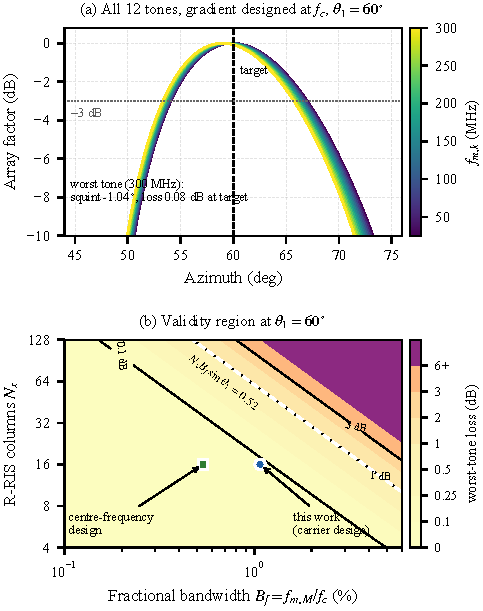
\includegraphics[width=0.9\columnwidth]{F4rev_multitone_beam}
\caption{(a) Array factor of all $M=12$ tones for an \Rris{} gradient designed at $f_c$ and steered to $\theta_1=60^\circ$; the worst tone squints by $-1.04^\circ$ and loses 0.08\,dB toward the target. (b) Worst-tone loss toward the target versus fractional bandwidth and number of \Rris{} columns at $\theta_1=60^\circ$; the dashed line $N_xB_f\sin\theta_1=0.52$ is the 1-dB boundary.}
\label{fig:beamforming}
\end{figure}

\subsection{Multi-Tone Beam Coherence}
\label{sec:squint}
Because the \Rris{} gradient \eqref{eq:psi} is phase-only and designed at a single frequency $f_d$ (the carrier, $f_d = f_c$, unless stated otherwise), tone $k$ at $f_k = f_d + f_{m,k}$ is steered to $\theta_k = \arcsin(\sin\theta_1\,f_d/f_k)$, i.e., squinted by~\cite{mailloux2017phased}
\begin{equation}
\Delta\theta_k = \arcsin\!\left(\sin\theta_1\,\frac{f_d}{f_d+f_{m,k}}\right) - \theta_1
\approx -\tan\theta_1\,\frac{f_{m,k}}{f_d}.
\label{eq:squint}
\end{equation}
For the worst tone ($f_{m,M} = 300$\,MHz) at $\theta_1 = 60^\circ$, $\Delta\theta_M = -1.04^\circ$, 8.2\,\% of the 12.7$^\circ$ HPBW of the 16-column aperture [Fig.~\ref{fig:beamforming}(a)]; the array-factor peaks agree with \eqref{eq:squint} to within $0.01^\circ$ at every scan angle tested. The tones therefore point in slightly different directions, but all remain inside the 3-dB beam. The gain toward the target falls by 0.08\,dB for the worst tone and by 0.03\,dB averaged over the tones; this raises $\sqrt{\mathrm{CRB}(R_{\mathrm{tot}})}$ by 0.4\,\% and, because the symmetric aperture keeps every tone gain real, produces no range bias (Table~S2). The squint grows relative to the HPBW with scan angle, from 4.8\,\% at $30^\circ$ to 8.7\,\% at $75^\circ$.

Since the HPBW of an $N_x$-column half-wavelength aperture is $\approx 1.772/(N_x\cos\theta_1)$\,rad, the worst-tone loss depends on the product $N_x B_f \sin\theta_1$, where $B_f = f_{m,M}/f_d$ is the fractional bandwidth. The exact array factor [Fig.~\ref{fig:beamforming}(b)] places the 1-dB worst-tone loss at $N_x B_f \sin\theta_1 = 0.52$; the present design operates at 0.15. One symbol-independent gradient therefore suffices whenever $N_x B_f\sin\theta_1 \lesssim 0.5$. For larger apertures or bandwidths ($N_x = 64$ would lose 1.3\,dB), designing the gradient at the comb centre, $f_d = f_c + (f_{m,1}+f_{m,M})/2$, halves the maximum squint (0.49$^\circ$ at $60^\circ$) at no cost. A single-stage STM-RIS re-steered every symbol avoids squint altogether, but only by reloading $M$ phase maps per sweep, which is the overhead the two-stage design removes.

\subsection{Bistatic Signal Model}
The power incident on the RIS is
\begin{equation}
P_{\mathrm{ap}} = \frac{P_{\mathrm{Tx}} G_{\mathrm{Tx}} A_{\mathrm{RIS}}}
{4\pi d_{TR}^2},
\label{eq:Pap}
\end{equation}
where $A_{\mathrm{RIS}}$ is the effective \Tris{} aperture. Accounting for
the \Tris{} conversion efficiency into the harmonic $f_{m,k}$, the near-field
inter-stage coupling power and the \Rris{} reflection efficiency, the
equivalent radiated power at the harmonic during symbol $k$ is
\begin{equation}
P_{\mathrm{RIS}}(k) = \frac{|T_{\mathrm{sb}}(f)|^2}{2}\,
C_0^2\,|\Gamma|^2\, P_{\mathrm{ap}}.
\label{eq:Pris}
\end{equation}
Treating the RIS as a transmitter with harmonic-dependent directive gain
$G_{\mathrm{RIS}}^{(k)}(\theta_1)$ and applying the bistatic radar equation,
the received power at the Rx after target scattering
is~\cite{willis2005bistatic,tang2020wireless}
\begin{equation}
P_{\mathrm{rx}}(k) =
\frac{P_{\mathrm{Tx}} G_{\mathrm{Tx}} A_{\mathrm{RIS}}
\frac{|T_{\mathrm{sb}}(f)|^2}{2} C_0^2 |\Gamma|^2
G_{\mathrm{RIS}}^{(k)}(\theta_1) G_{\mathrm{rx}} \lambda^2 \sigma_{\mathrm{RCS}}}
{(4\pi)^4 d_{TR}^2 R_{\mathrm{ris\text{-}t}}^2 R_{\mathrm{t\text{-}rx}}^2},
\label{eq:Prx}
\end{equation}
where $\lambda_k = c/(f_c + f_{m,k})$. This expression links the Tx power,
RIS aperture, harmonic conversion and beam gain to the expected per-symbol
received energy. With positions $\bm{x}_{\mathrm{tx}}$, $\bm{x}_{\mathrm{ris}}$,
$\bm{x}_{\mathrm{rx}}$ and target $\bm{x}(t)$, the total Tx-to-Rx
propagation delay is
\begin{equation}
\tau_{\mathrm{tot}} = \frac{R_{\mathrm{tx\text{-}ris}} +
R_{\mathrm{ris\text{-}t}} + R_{\mathrm{t\text{-}rx}}}{c},
\label{eq:tau}
\end{equation}
with
\begin{align}
R_{\mathrm{tx\text{-}ris}} &= \|\bm{x}_{\mathrm{tx}} - \bm{x}_{\mathrm{ris}}\| = d_{TR},
\label{eq:R1}\\
R_{\mathrm{ris\text{-}t}} &= \|\bm{x}_{\mathrm{ris}} - \bm{x}\|,
\label{eq:R2}\\
R_{\mathrm{t\text{-}rx}} &= \|\bm{x} - \bm{x}_{\mathrm{rx}}\|.
\label{eq:R3}
\end{align}
In M-FSK radar the transmitter steps sequentially through all $M$ tones,
radiating each for one symbol period $T_{\mathrm{sym}}$ before stepping to
the next. One complete cycle constitutes a sweep of duration
\begin{equation}
T_{\mathrm{sw}} = M\,T_{\mathrm{sym}},
\label{eq:Tsw}
\end{equation}
and the CPI consists of $N_{\mathrm{sw}}$ sweeps, with total duration
$T_{\mathrm{CPI}} = N_{\mathrm{sw}} T_{\mathrm{sw}}$. The slow-time index
$p \in \{1,\dots,N_{\mathrm{sw}}\}$ counts sweeps, with timestamp
$t_p = p\,T_{\mathrm{sw}}$. The absolute frequency of tone $k$ is
\begin{equation}
f_k = f_c + f_{m,k}.
\label{eq:fk}
\end{equation}
Letting $\xi_{lk}$ denote the per-element phase at Rx element $l$ for tone
$k$ (incorporating the RIS beamforming phase and propagation offset), the
complex baseband sample at Rx element $l$, tone $k$, sweep $p$ is
\begin{equation}
r_l(k,p) = A_k \exp\!\big\{j\big[-2\pi f_{m,k}\tau_{\mathrm{tot}}
+ 2\pi f_D(k)\,t_{kp} + \xi_{lk}\big]\big\},
\label{eq:rlkp}
\end{equation}
where $A_k = \sqrt{2P_{\mathrm{rx}}(k)}$ from \eqref{eq:Prx} and $f_D(k)$ is
the instantaneous bistatic Doppler frequency. Here $t_{kp} = t_p + (k-1)T_{\mathrm{sym}}$ is the sampling instant of tone $k$ in sweep $p$; the intra-sweep offset $(k-1)T_{\mathrm{sym}}$ couples Doppler into the tone phases and is compensated in Section~\ref{sec:range_est}.
Defining the unit vectors
\begin{align}
\bm{u}_{\mathrm{rt}} &= (\bm{x} - \bm{x}_{\mathrm{ris}})/
\|\bm{x} - \bm{x}_{\mathrm{ris}}\|,
\label{eq:urt}\\
\bm{u}_{\mathrm{rx,t}} &= (\bm{x}_{\mathrm{rx}} - \bm{x})/
\|\bm{x}_{\mathrm{rx}} - \bm{x}\|,
\label{eq:urxt}
\end{align}
the Doppler frequency for tone $k$ is
\begin{equation}
f_D(k) \approx -\frac{f_k}{c}\big(\bm{u}_{\mathrm{rt}} - \bm{u}_{\mathrm{rx,t}}\big)\!\cdot\!\bm{v}.
\label{eq:fd}
\end{equation}
Here $(\bm{u}_{\mathrm{rt}} - \bm{u}_{\mathrm{rx,t}})\!\cdot\!\bm{v} = \dot L$ is the rate of the bistatic path $L = R_{\mathrm{ris\text{-}t}} + R_{\mathrm{t\text{-}rx}}$, so that $f_D(k) = -\dot L/\lambda_k$.
With additive noise $n_l(k,p) \sim \mathcal{CN}(0,\sigma_n^2)$, the received
sample is
\begin{equation}
y_l(k,p) = r_l(k,p) + n_l(k,p),
\label{eq:ylkp}
\end{equation}
and Rx beamforming with steering weights $a_l$ over $N_{\mathrm{rx}}$
elements yields
\begin{equation}
y_{\mathrm{bf}}(k,p) = \sum_{l=1}^{N_{\mathrm{rx}}} a_l^*\, y_l(k,p).
\label{eq:ybf}
\end{equation}
Range, velocity and angle are estimated over one CPI: range from a
stepped-frequency Inverse Fast Fourier Transform (IFFT) over the $M$ tones, velocity from a slow-time FFT over
the $N_{\mathrm{sw}}$ sweeps and angle from the $N_{\mathrm{rx}}\times 1$
spatial snapshot formed, after range and Doppler estimation, by phase-aligning and summing all $MN_{\mathrm{sw}}$ samples at each element,
\begin{equation}
[\bm{y}_{\mathrm{snap}}]_l = \sum_{k=1}^{M}\sum_{p=1}^{N_{\mathrm{sw}}} y_l(k,p)\,
e^{\,j2\pi[f_{m,k}\hat{\tau}_{\mathrm{tot}} - \hat f_D(k)\,\tilde t_{kp}]},
\label{eq:ysnap}
\end{equation}
with $\tilde t_{kp}$ the sampling instant referred to the CPI centre. Its post-beamforming SNR is $\mathrm{SNR}_{\mathrm{snap}} = M\,\mathrm{SNR}_{\mathrm{CPI}}$.

\begin{figure}[!t]
\centering
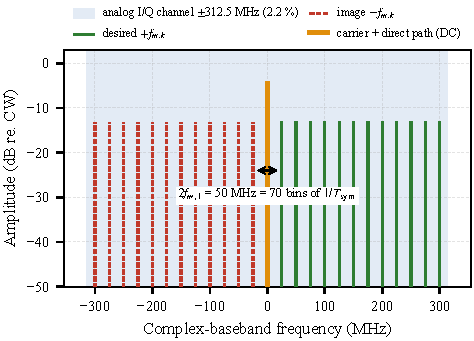
\includegraphics[width=0.9\columnwidth]{F3rev_baseband_spectrum}
\caption{Per-symbol complex-baseband spectrum at the Rx after I/Q down-conversion with the local oscillator at $f_c$, referenced to the incident CW. Desired tones occupy $+f_{m,k}$ and images $-f_{m,k}$ ($-13.2$\,dB each); the carrier feedthrough and the direct Tx path fall at DC ($-4.5$\,dB). Because $\Delta f\,T_{\mathrm{sym}}=35$ is an integer, tones, images and carrier are mutually orthogonal over one symbol.}
\label{fig:mfsk_spectrum}
\end{figure}

\subsection{Sideband Separation in the Complex-Baseband Receiver}
\label{sec:sideband}
Because the \Rris{} phase gradient is frequency-independent, the image at $f_c-f_{m,k}$ is steered to within $1.09^\circ$ of $\theta_1$, on the side opposite to the desired tone, and returns from the target with it; unlike in a single-stage STM-RIS, where it is steered to $-\theta_1$, it cannot be rejected spatially. It is instead separated in the receiver. After quadrature (I/Q) down-conversion with the local oscillator at $f_c$, which \eqref{eq:rlkp}--\eqref{eq:ybf} already presuppose, the desired tone and its image occupy $+f_{m,k}$ and $-f_{m,k}$, opposite halves of the complex-baseband spectrum, while the carrier feedthrough and the direct Tx path fall at DC (Fig.~\ref{fig:mfsk_spectrum}). The sample of tone $k$ is formed by correlating one symbol with $e^{-j2\pi f_{m,k}t}$. Since $\Delta f\,T_{\mathrm{sym}} = 35$ is an integer, every tone, every image and the carrier complete an integer number of cycles in $T_{\mathrm{sym}}$ and are mutually orthogonal: the nearest image lies $2f_{m,1}T_{\mathrm{sym}} = 70$ correlator bins away, rather than 0.18\,\% away at radio frequency. The analog front end therefore needs only a $\pm312.5$\,MHz channel filter (2.2\,\% fractional bandwidth); no high-$Q$ sideband filter is required.

The residual coupling is quadrature imbalance. Writing the received baseband signal as $\mu x + \nu x^{*}$, with Q-branch gain ratio $g$ and phase error $\phi$, the image-rejection ratio is
\begin{equation}
\mathrm{IRR} = \frac{|\mu|^2}{|\nu|^2} = \frac{1+2g\cos\phi+g^2}{1-2g\cos\phi+g^2}.
\label{eq:irr}
\end{equation}
Because the image returns from the same target, its leakage onto $+f_{m,k}$ carries the target delay slope across the tones but the conjugate slow-time Doppler. It therefore causes no range bias; it produces only a Doppler-mirror ghost at $(R_{\mathrm{tot}}, -v)$, $\mathrm{IRR}$\,dB below the target. Keeping this ghost below the noise of one range--Doppler cell requires $\mathrm{IRR} > \mathrm{SNR}_{\mathrm{CPI}} + 10\log_{10}M = 26.4$\,dB. For an assumed imbalance of 0.2\,dB and $1^\circ$, \eqref{eq:irr} gives 36.8\,dB, a 10.4\,dB margin [Fig.~S1(a)]. A time-domain simulation of the correlator reproduces \eqref{eq:irr} to within 0.01\,dB and confirms both the ghost level and the absence of a range shift.

Separating the sidebands digitally moves the hardware requirement to the \Tris{} modulator, which must follow the DDS drive up to $f_{m,M} = 300$\,MHz. Modelling the diode and its bias network as a first-order response with effective time constant $\tau_{\mathrm{sw}}$, a sideband loss below 1\,dB at $f_{m,M}$ requires $\tau_{\mathrm{sw}} \le 0.27$\,ns [Fig.~S1(b)]. Offsetting the tone comb to $f_{m,k} = f_{\mathrm{off}} + k\Delta f$ would widen the radio-frequency guard band without changing the resolution or the CRB, but would tighten this requirement (Table~S1); the unoffset comb is therefore retained.

\begin{table}[!t]
\centering
\caption{Tracking Scenario and Performance (Straight Line)}
\label{tab:tracking}
\footnotesize
\setlength{\tabcolsep}{2pt}
\begin{tabular}{@{}lcc@{}}
\hline\hline
Parameter & Symbol & Value \\
\hline
Initial range / angle & $R_0$, $\theta_0$ & 10 m, 60$^\circ$ \\
Target speed / heading & $|\bm v|$, $\psi_v$ & 2.0 m/s, 45$^\circ$ \\
Final range / angle (frame 50) & $R_{50}$, $\theta_{50}$ & 11.65 m, 57.83$^\circ$ \\
CPIs / duration & $N_{\rm fr}$, $T_{\rm tot}$ & 50, 860.2 ms \\
Rx bistatic angle & $\beta$ & 60$^\circ$ \\
\hline
\end{tabular}\\[2pt]
\begin{tabular}{@{}lccc@{}}
Metric & Per-CPI fix & $\alpha$-smoother & IMM \\
\hline
Position RMSE & 2.76 cm & 2.56 cm & 0.97 cm \\
95th-pct position error & 5.09 cm & 4.05 cm & 1.87 cm \\
Velocity RMSE & -- & -- & 5.26 cm/s \\
Pointing error (rms) & 0.134$^\circ$ & 0.154$^\circ$ & 0.051$^\circ$ \\
Mean illumination loss & 0.001 dB & 0.002 dB & 0.000 dB \\
\hline\hline
\multicolumn{4}{@{}p{0.97\columnwidth}@{}}{\scriptsize 200 Monte Carlo trials; $\mathrm{SNR}_1=-14.5$\,dB at the start; measurement noise at the corrected bounds of the frame SNR, including the illumination gain of the beam commanded one CPI earlier.}
\end{tabular}
\end{table}

\section{Target Sensing and Tracking}
\label{sec:tracking}
In the bistatic deployment, the \Rris{} beam must continuously track a moving
target by updating the \Rris{} phase map as the target azimuth changes over
successive CPIs. This section presents the angle, range and velocity
estimators with their CRBs, the bistatic geometry inversion and the tracking filters. Tracking parameters are listed in
Table~\ref{tab:tracking}.

\subsection{Rx-Array Angle Estimation}
The bistatic Rx array is centered at the fixed position
$\bm{p}_{\mathrm{rx}}$, with broadside along the bearing $\theta_b$ of the surveillance region. Its steering vector toward azimuth $\theta$ is
\begin{equation}
\bm{a}_{\mathrm{rx}}(\theta) =
\big[1,\, e^{j\kappa\sin(\theta-\theta_b)},\,\dots,\,
e^{j(N_{\mathrm{rx}}-1)\kappa\sin(\theta-\theta_b)}\big]^T,
\label{eq:arx}
\end{equation}
with $\kappa = 2\pi d_{\mathrm{rx}}/\lambda$.
The angle-of-arrival $\hat{\theta}_{\mathrm{Rx}\to t}$ is estimated by
maximizing the conventional (matched-filter) beamformer
output~\cite{van2002optimum, krim2002two}
\begin{equation}
\hat{\theta}_{\mathrm{Rx}\to t} =
\argmax_\theta \big|\bm{a}_{\mathrm{rx}}(\theta)^H
\bm{y}_{\mathrm{snap}}\big|^2.
\label{eq:theta_est}
\end{equation}
The CRB for the angle, for a deterministic signal with unknown complex amplitude, is~\cite{van2002optimum, steven1993fundamentals}
\begin{equation}
\mathrm{CRB}(\theta_{\mathrm{Rx}\to t}) =
\frac{6}{\kappa^2\cos^2\!\varphi_t\,(N_{\mathrm{rx}}^2-1)\,\mathrm{SNR}_{\mathrm{snap}}},
\label{eq:crb_theta}
\end{equation}
where $\varphi_t = \theta_{\mathrm{Rx}\to t}-\theta_b$ and $\mathrm{SNR}_{\mathrm{snap}} = M\,\mathrm{SNR}_{\mathrm{CPI}}$ is the SNR of the snapshot \eqref{eq:ysnap}; at the operating point $\sqrt{\mathrm{CRB}} = 0.134^\circ$. The beam scan \eqref{eq:theta_est} is evaluated on a $0.5^\circ$ grid and its peak refined by parabolic interpolation and Newton iterations.

\subsection{Range Estimation}
\label{sec:range_est}
The total bistatic path is estimated from the $M$ complex phasors obtained by Doppler-compensated coherent averaging of \eqref{eq:ybf} for each tone,
\begin{equation}
\bar{y}(k) = \frac{1}{N_{\mathrm{sw}}}
\sum_{p=1}^{N_{\mathrm{sw}}} y_{\mathrm{bf}}(k,p)\,e^{-j2\pi \hat f_D(k)\,\tilde t_{kp}},
\label{eq:ybar}
\end{equation}
where $\tilde t_{kp}$ is $t_{kp}$ referred to the CPI centre and $\hat f_D(k) = \hat f_D f_k/f_c$ uses the Doppler estimate of Section~\ref{sec:vel_est}. The compensation removes the slow-time rotation, its tone dependence and the intra-sweep term, so the path estimate refers to the mid-CPI position; averaging sweep powers instead forfeits the coherent gain on which \eqref{eq:crb_R} is based.
A zero-padded IFFT of $[\bar{y}(1),\dots,\bar{y}(M)]$ yields a range profile
whose peak encodes $\tau_{\mathrm{tot}}$. For an IFFT length $N_{\mathrm{FFT}}$, the profile is sampled on a grid of spacing~\cite{richards2005fundamentals,rohling2001waveform}
\begin{equation}
\delta R = \frac{c}{N_{\mathrm{FFT}}\,\Delta f},
\label{eq:dR}
\end{equation}
whereas the Rayleigh resolution of the $M$-tone aperture is $c/(M\Delta f) = 1.0$\,m. The IFFT returns a wrapped estimate $R_{\mathrm{wrap}}$ modulo the unambiguous path $c/\Delta f = 11.99$\,m; the true path is recovered as
\begin{equation}
R_{\mathrm{tot}} = R_{\mathrm{wrap}} + n_{\mathrm{amb}}\,c/\Delta f,
\label{eq:Rtot}
\end{equation}
where $n_{\mathrm{amb}}$ is resolved from coarse prior knowledge at acquisition. The integer peak of the profile is refined by parabolic interpolation of the three samples around the maximum and then by Newton iterations on the periodogram, i.e., the single-target maximum-likelihood estimate
\begin{equation}
\hat R_{\mathrm{tot}} = \argmax_R \Big|\sum_{k=1}^{M} \bar y(k)\,e^{j2\pi f_{m,k}R/c}\Big|^2.
\label{eq:R_ml}
\end{equation}
With $N_{\mathrm{FFT}}=8M$, argmax alone is limited by the grid, $\delta R/\sqrt{12} = 3.6$\,cm, which interpolation removes (Section~\ref{sec:efficiency}).
 The CRB for total-path estimation from $M$ coherently combined
tones is~\cite{rohling2001waveform}
\begin{equation}
\mathrm{CRB}(R_{\mathrm{tot}}) =
\frac{c^2}{8\pi^2 \sigma_f^2\, M\, \mathrm{SNR}_{\mathrm{CPI}}},
\label{eq:crb_R}
\end{equation}
where $\sigma_f^2$ is the variance of the tone frequencies about their mean and $\mathrm{SNR}_{\mathrm{CPI}} = N_{\mathrm{sw}}\mathrm{SNR}_1$ is the per-tone SNR after coherent integration; at the operating point $\sqrt{\mathrm{CRB}(R_{\mathrm{tot}})} = 1.87$\,cm.

\subsection{Velocity Estimation}
\label{sec:vel_est}
The Doppler estimate is obtained from the slow-time sequence $y_{\mathrm{bf}}(k,p)$, with the $M$ magnitude spectra of a $4\times$ zero-padded FFT averaged to suppress noise:
\begin{equation}
\hat{f}_D = \argmax_f \frac{1}{M}\sum_k
\Big|\sum_{p} y_{\mathrm{bf}}(k,p)\,e^{-j2\pi f (f_k/f_c)\tilde t_{kp}}\Big|^2,
\label{eq:fd_est}
\end{equation}
evaluated on the FFT grid and refined, as for range, by parabolic interpolation and Newton iterations. The Doppler resolution $\delta f_D = 1/T_{\mathrm{CPI}}$ sets the FFT grid but not the accuracy of the refined estimate. Over the $MN_{\mathrm{sw}}$ sampling instants the CRB is~\cite{harris1978use,steven1993fundamentals, willis2005bistatic}
\begin{equation}
\mathrm{CRB}(f_D) = \frac{3}{2\pi^2 M\,T_{\mathrm{CPI}}^2\, \mathrm{SNR}_{\mathrm{CPI}}},
\label{eq:crb_fd}
\end{equation}
and the radial velocity $v = \lambda f_D/2$ (half the bistatic path rate) has $\sqrt{\mathrm{CRB}} = 0.58$\,cm/s at the operating point.

\subsection{Positioning CRB}
Given $\hat{\theta}_{\mathrm{Rx}\to t}$ and the bistatic path $L = R_{\mathrm{tot}} - R_{\mathrm{tx\text{-}ris}}$ (the Tx--RIS leg is fixed and known), the target position is recovered from the intersection of the Rx line-of-bearing and the bistatic ellipse with foci at the RIS and the Rx
~\cite{willis2005bistatic, willis2007advances}. The
bearing unit vector is
\begin{equation}
\hat{\bm{u}} = [\sin\theta_{\mathrm{Rx}\to t},\,
\cos\theta_{\mathrm{Rx}\to t}]^T,
\label{eq:u}
\end{equation}
and the scalar Rx-to-target distance along $\hat{\bm{u}}$ is
\begin{equation}
r = \frac{L^2 - \|\bm{a}\|^2}{2(\bm{a}\!\cdot\!\hat{\bm{u}} + L)},
\label{eq:r}
\end{equation}
where $\bm{a} = \bm{p}_{\mathrm{rx}} - \bm{p}_{\mathrm{RIS}}$ is the Rx-RIS
baseline. The estimated target position and required beam angle are
\begin{align}
(x_T, y_T) &= \bm{p}_{\mathrm{rx}} + r\hat{\bm{u}},
\label{eq:pos}\\
\theta_{\mathrm{cmd}} &= \operatorname{atan2}(x_T, y_T).
\label{eq:theta2}
\end{align}
Propagating the path and angle bounds through \eqref{eq:u}--\eqref{eq:pos} with the Jacobian $\bm{J} = \partial(x_T,y_T)/\partial(L,\theta_{\mathrm{Rx}\to t})$ gives~\cite{steven1993fundamentals}
\begin{equation}
\mathrm{CRB}_{\mathrm{pos}} = \mathrm{tr}\big\{\bm{J}\,\mathrm{diag}\big(\mathrm{CRB}(L),\mathrm{CRB}(\theta_{\mathrm{Rx}\to t})\big)\,\bm{J}^T\big\}.
\label{eq:crb_pos}
\end{equation}
Along the line of bearing $\partial r/\partial L = 1/(1+\cos\beta)$, where $\beta$ is the bistatic angle at the target, so the path error is amplified without bound as $\beta \to 180^\circ$ (forward scatter). With the Rx at $\beta = 60^\circ$ (Table~\ref{tab:sys_params}), $\|\partial(x_T,y_T)/\partial L\| = 0.67$ and $\sqrt{\mathrm{CRB}_{\mathrm{pos}}} = 2.49$\,cm; at $\beta = 155^\circ$ the path error would be amplified $10.9\times$ and $\sqrt{\mathrm{CRB}_{\mathrm{pos}}} = 22.3$\,cm.

\subsection{Target Tracking}
The \Rris{} beam must point at the target one $T_{\mathrm{CPI}}$ ahead. Each CPI yields a position fix $\bm{z}_p$ from \eqref{eq:u}--\eqref{eq:pos}, with covariance $\bm{R}_p = \bm{J}\,\mathrm{diag}\big(\mathrm{CRB}(L),\mathrm{CRB}(\theta_{\mathrm{Rx}\to t})\big)\bm{J}^T$, and a bistatic path-rate measurement $\hat{\dot L} = -\lambda\hat f_D$ with variance $4\,\mathrm{CRB}(v)$. With state $\bm{x} = [\bm{p}^T, \bm{v}^T]^T$ for constant velocity (CV) or $[\bm{p}^T,\bm{v}^T,\bm{a}^T]^T$ for constant acceleration (CA), the measurement model is
\begin{equation}
\bm{z} = \begin{bmatrix}\bm{z}_p\\ \hat{\dot L}\end{bmatrix}
= \begin{bmatrix}\bm{p}\\ (\bm{u}_{\mathrm{rt}}-\bm{u}_{\mathrm{rx,t}})\cdot\bm{v}\end{bmatrix} + \bm{n},
\label{eq:meas}
\end{equation}
whose Doppler row is linearized about the predicted state in an extended Kalman filter (EKF)~\cite{bar2001estimation}. Manoeuvres are handled by an interacting multiple-model (IMM) filter that mixes a CV EKF (process noise 0.2\,m/s$^2$) and a CA EKF (30\,m/s$^3$) with a mode-switching probability of 0.05 per CPI~\cite{bar2001estimation,blackman1999design}. The beam command for the next CPI is the bearing of the predicted position,
\begin{equation}
\theta_{\mathrm{pred}} = \operatorname{atan2}(x_{\mathrm{pred}}, y_{\mathrm{pred}}),
\label{eq:theta_pred}
\end{equation}
loaded to the \Rris{} via SPI. As baselines, a first-order $\alpha$-smoother ($\alpha = 0.3$) applied directly to the per-CPI bearing without prediction, an $\alpha$--$\beta$ filter on the fixes, and single-model CV and CA EKFs are also evaluated.

\section{RIS-Enabled M-FSK Sensing}
\label{sec:results}

\begin{figure}[!t]
\centering
\subfloat[Transmission amplitude]{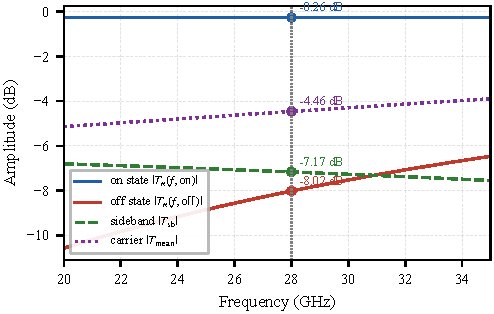
\includegraphics[width=0.8\columnwidth]{F2a_transmission_amplitude}\label{fig:pin_a}}
\hfil
\subfloat[Phase response]{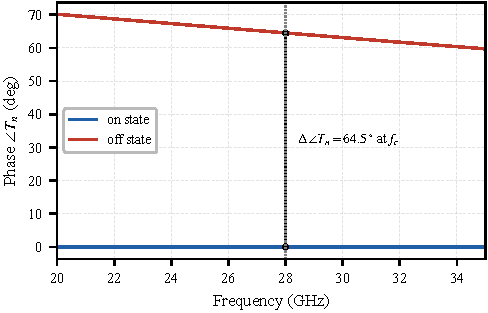
\includegraphics[width=0.8\columnwidth]{F2b_phase_response}\label{fig:pin_b}}
\\ \vspace{0.5em}
\subfloat[Impedance magnitude]{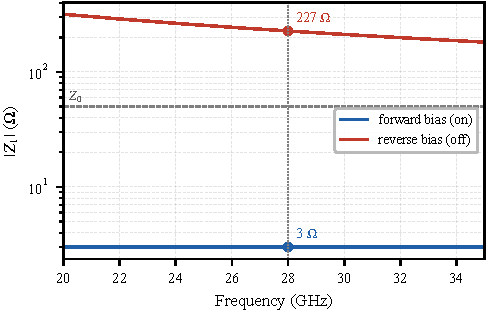
\includegraphics[width=0.8\columnwidth]{F2c_impedance_magnitude}\label{fig:pin_c}}
\caption{\Tris{} PIN-diode element response versus frequency from the
equivalent-circuit model \eqref{eq:diode_Z}-\eqref{eq:Tn}. (a) Transmission
amplitude $|T_n|$ in the on- and off-states; the carrier ($f_c=28$\,GHz) is
marked. (b) Transmission phase $\angle T_n$, with a $64.5^\circ$ on/off
difference at $f_c$. (c) Element impedance magnitude $|Z_1|$ for forward and
reverse bias.}
\label{fig:pin_diode}
\end{figure}

\subsection{T-RIS Phase Control and R-RIS Beamforming}
Fig.~\ref{fig:pin_diode} characterizes the \Tris{} element transmission over
20-35\,GHz, derived from the PIN-diode equivalent circuit
\eqref{eq:diode_Z} with $R_s = 2\,\Omega$ and $C_J = 25$\,fF. In the
on-state [Fig.~\ref{fig:pin_diode}(a)], $Z_1(f,\mathrm{on}) = 3\,\Omega \ll
Z_0$, placing the diode in a near-short condition with
$|T_n(f,\mathrm{on})| = -0.26$\,dB. In the off-state,
$|Z_1(f,\mathrm{off})| = 227\,\Omega$ at 28\,GHz and
$|T_n(f,\mathrm{off})| = -8.02$\,dB, yielding a sideband coefficient
$|T_{\mathrm{sb}}| = -7.17$\,dB and a carrier feedthrough
$|T_{\mathrm{mean}}| = -4.46$\,dB. The sideband coefficient varies by less
than 0.4\,dB across 20-35\,GHz, confirming a flat modulation efficiency
over the 12-tone waveform. Fig.~\ref{fig:pin_diode}(b) shows the on-state
phase $\angle T_n(\mathrm{on}) \approx 0^\circ$ (near-resistive load) and
the off-state phase $\angle T_n(\mathrm{off}) = +64.5^\circ$, arising from
the capacitive reactance of $C_J$ under reverse bias.
Fig.~\ref{fig:pin_diode}(c) shows the on-state impedance to be flat and
resistive ($\approx R_s$), while the off-state impedance falls from above
300\,$\Omega$ at 20\,GHz to 227\,$\Omega$ at 28\,GHz as the capacitive
reactance decreases with frequency. These values are consistent with
reported mmWave PIN-diode specifications~\cite{dai2020reconfigurable,hillerdesign}.

Fig.~\ref{fig:mfsk_spectrum} shows the per-symbol spectrum seen by the complex-baseband receiver. The twelve desired tones occupy $+f_{m,k} \in \{25,\dots,300\}$\,MHz and the twelve co-steered images $-f_{m,k}$, each $-13.2$\,dB relative to the incident CW, while the carrier feedthrough and the direct Tx path fall at DC ($-4.5$\,dB). All of them are orthogonal over one symbol, so the per-symbol correlator isolates each desired tone; the residual coupling is set by the quadrature imbalance analysed in Section~\ref{sec:sideband}.

The \Rris{} is a $16\times16$ uniform planar array with half-wavelength spacing. Steered to $\theta_1 = 60^\circ$ with 3-bit phase quantization, it has HPBW $\approx 13^\circ$ and a first sidelobe level of $-13.3$\,dB; the quantized gradient offsets the peak by a fixed 0.87$^\circ$, which can be pre-compensated, and costs 0.22\,dB of gain (Section~\ref{sec:phase_noise}). Fig.~\ref{fig:beamforming}(a) shows that all twelve tones remain within the 3-dB beam (Section~\ref{sec:squint}).

\begin{figure}[!t]
\centering
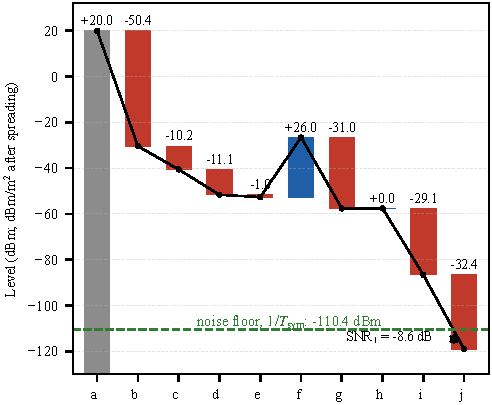
\includegraphics[width=0.95\columnwidth]{F5rev_link_budget}
\caption{Link budget \eqref{eq:Prx} at the operating geometry: cumulative level after each stage (power in dBm, power density in dBm/m$^2$ after spreading). The received power per tone lies 8.6\,dB below the per-symbol noise floor ($\mathrm{SNR}_1 = -8.6$\,dB); the system is evaluated at $\mathrm{SNR}_1 = -14.5$\,dB.}
\label{fig:link_budget}
\end{figure}

\subsection{RIS-M-FSK Target Sensing}
\label{sec:linkbudget}
Fig.~\ref{fig:link_budget} evaluates the link budget \eqref{eq:Prx} for the operating geometry. The RIS aperture ($A = 73.4$\,cm$^2$) captures -50.4\,dB of the 20\,dBm radiated by the Tx at $d_{TR} = 8$\,m. Sideband conversion ($|T_{\mathrm{sb}}|^2/2$, -10.2\,dB), inter-stage coupling ($C_0^2$, -11.1\,dB, Section~\ref{sec:5b}) and \Rris{} reflection ($|\Gamma|^2$, -1.0\,dB) set the power re-radiated at $f_c + f_{m,k}$, which the \Rris{} aperture gain toward $\theta_1$, $4\pi A\cos\theta_1/\lambda^2 = 26.0$\,dBi, directs toward the target. After spreading to the target and to the Rx, a 0\,dBsm RCS and the Rx aperture $G_{\mathrm{Rx}}\lambda^2/(4\pi)$ (-32.4\,dB), the received power per tone is -119.0\,dBm. The per-symbol correlator of Section~\ref{sec:sideband} integrates each tone over $T_{\mathrm{sym}}$, so the noise bandwidth is $1/T_{\mathrm{sym}} = 714$\,kHz and the noise floor $k T_0 F/T_{\mathrm{sym}} = -110.4$\,dBm, giving $\mathrm{SNR}_1 = -8.6$\,dB. We evaluate the system at $\mathrm{SNR}_1 = -14.5$\,dB, which reserves 5.9\,dB for implementation losses not modelled here, such as feed and connector losses, oscillator and converter noise, and polarization mismatch. Coherent integration over $N_{\mathrm{sw}} = 1024$ sweeps adds 30.1\,dB, giving $\mathrm{SNR}_{\mathrm{CPI}} = 15.6$\,dB per tone, and the coherent combination of the $M = 12$ tones adds a further 10.8\,dB.

\begin{figure}[!t]
\centering
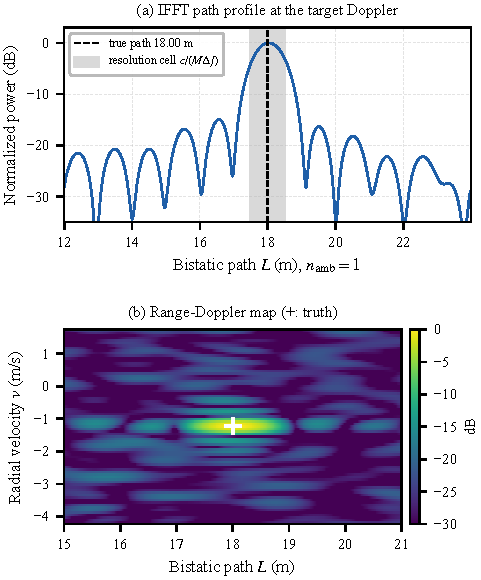
\includegraphics[width=0.9\columnwidth]{F6rev_range_doppler}
\caption{Single-target detection at $\mathrm{SNR}_1 = -14.5$\,dB for the geometry of Table~\ref{tab:sys_params}. (a) IFFT path profile at the target Doppler, unwrapped with $n_{\mathrm{amb}} = 1$; the shaded band is the $c/(M\Delta f) = 1$\,m resolution cell. (b) Range--Doppler map.}
\label{fig:range_doppler}
\end{figure}

Fig.~\ref{fig:range_doppler} shows the IFFT path profile and the range--Doppler map for the target of Table~\ref{tab:sys_params}: bistatic path 18.00\,m and radial velocity -1.22\,m/s. The profile, unwrapped with $n_{\mathrm{amb}} = 1$, peaks within the 1\,m resolution cell, and the refined estimate lies 2.4\,cm and 0.6\,cm/s from the truth, confirming joint path--velocity estimation within one CPI.

\begin{figure}[!t]
\centering
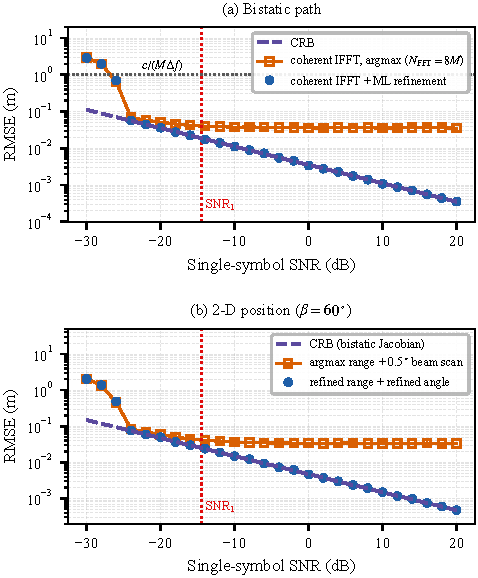
\includegraphics[width=0.9\columnwidth]{F7rev_rmse_path_position}
\caption{Monte Carlo RMSE (1000 trials) versus single-symbol SNR for (a) the bistatic path and (b) the 2-D position at $\beta=60^\circ$, with the bounds \eqref{eq:crb_R} and \eqref{eq:crb_pos}. Squares: coherent IFFT argmax and $0.5^\circ$ beam scan; circles: with peak refinement. The operating point $\mathrm{SNR}_1=-14.5$\,dB is marked.}
\label{fig:rmse_range}
\end{figure}

\begin{figure}[!t]
\centering
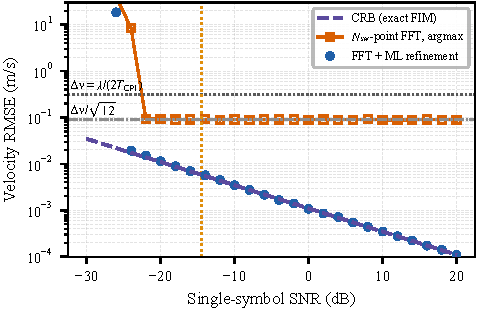
\includegraphics[width=0.9\columnwidth]{F8rev_rmse_velocity}
\caption{Velocity RMSE versus SNR for the $N_{\mathrm{sw}}$-point FFT argmax and the refined estimator, with the bound \eqref{eq:crb_fd}. The argmax saturates at $\Delta v/\sqrt{12}$; the refined estimate follows the bound from $\mathrm{SNR}_1\approx-24$\,dB upward.}
\label{fig:rmse_velocity}
\end{figure}

\begin{table}[!t]
\centering
\caption{Estimation Performance Summary at the Operating Point}
\label{tab:estimation_perf}
\footnotesize
\begin{tabular}{@{}lrl@{}}
\hline\hline
Metric & Value & Units \\
\hline
Operating single-symbol SNR & $-14.5$ & dB \\
Post-CPI SNR ($N_{\mathrm{sw}}$=1024) & $15.6$ & dB \\
Path resolution $c/(M\Delta f)$ & 1.00 & m \\
Unambiguous path $c/\Delta f$ & 11.99 & m \\
Velocity resolution $\lambda/(2T_{\mathrm{CPI}})$ & 31.12 & cm/s \\
CRB path $\sqrt{\mathrm{CRB}_L}$, \eqref{eq:crb_R} & 1.87 & cm \\
CRB velocity & 0.58 & cm/s \\
CRB angle & 0.134 & deg \\
CRB position ($\beta=60^\circ$) & 2.49 & cm \\
RMSE path: argmax / refined & 4.09 / 1.84 & cm \\
RMSE velocity: FFT / refined & 8.96 / 0.59 & cm/s \\
RMSE angle: 0.5$^\circ$ scan / refined & 0.200 / 0.134 & deg \\
RMSE position: coarse / refined & 4.26 / 2.45 & cm \\
Efficiency RMSE/CRB (path, refined) & 0.98 & -- \\
MC trials per SNR point & 1000 & -- \\
\hline\hline
\multicolumn{3}{@{}p{0.95\columnwidth}@{}}{\scriptsize Operating point $\mathrm{SNR}_1=-14.5$\,dB, $N_{\mathrm{sw}}=1024$, $M=12$; refined = coherent 2-D processing with ML peak refinement (Section~\ref{sec:efficiency}).}
\end{tabular}
\end{table}

Figs.~\ref{fig:rmse_range} and~\ref{fig:rmse_velocity} report the Monte Carlo (MC) RMSE over 1000 trials per SNR point against the bounds of Section~\ref{sec:tracking}. In every trial the path is drawn uniformly within one IFFT grid cell and the path rate within one Doppler bin, so that grid effects are averaged rather than evaluated at a favourable point. For the bistatic path [Fig.~\ref{fig:rmse_range}(a)], the argmax of the $8M$-point coherent IFFT saturates near the grid-quantization level $\delta R/\sqrt{12} = 3.6$\,cm, whereas the refined estimator follows \eqref{eq:crb_R} from $\mathrm{SNR}_1 \approx -24$\,dB upward: at the operating point its RMSE is 1.84\,cm against a 1.87\,cm bound. The 2-D position [Fig.~\ref{fig:rmse_range}(b)], obtained through the inversion \eqref{eq:u}--\eqref{eq:pos}, reaches 2.45\,cm against the 2.49\,cm Jacobian bound, and 4.26\,cm with argmax range and a $0.5^\circ$ beam scan. The angle estimate attains its bound, $0.134^\circ$, once the beam-scan peak is refined ($0.200^\circ$ without refinement).

The velocity estimator [Fig.~\ref{fig:rmse_velocity}] behaves in the same way. The $N_{\mathrm{sw}}$-point FFT argmax is limited by its bin width, $\Delta v/\sqrt{12} = 9.0$\,cm/s, at all SNRs, while the refined estimate reaches 0.59\,cm/s against the 0.58\,cm/s bound. The Doppler resolution $\Delta v = 31.12$\,cm/s therefore governs the separation of targets in velocity, not the accuracy of a single-target estimate. The complete summary is given in Table~\ref{tab:estimation_perf}.

\begin{figure}[!t]
\centering
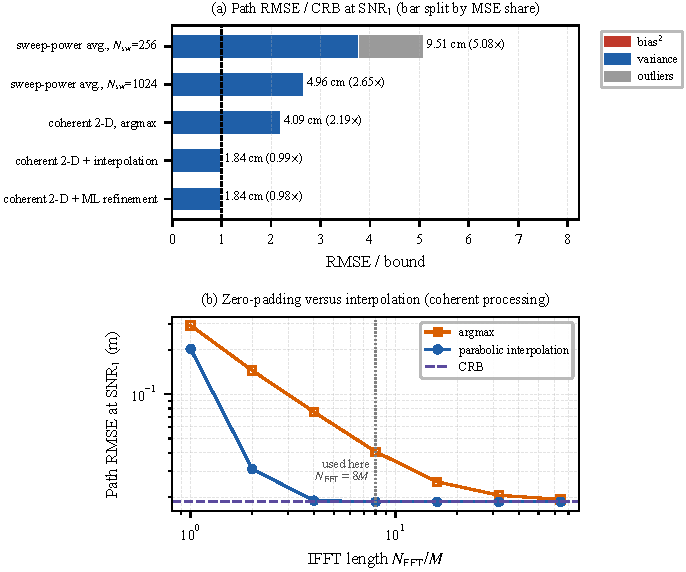
\includegraphics[width=0.9\columnwidth]{FA_estimator_efficiency}
\caption{Estimator efficiency at $\mathrm{SNR}_1=-14.5$\,dB. (a) Path RMSE relative to \eqref{eq:crb_R} for the estimators E1--E5 of Table~\ref{tab:error_budget}; each bar is split by the share of the MSE due to bias, variance and outliers ($|e|>0.5$\,m). (b) Path RMSE versus IFFT length with argmax and with parabolic interpolation; the truth is drawn uniformly over a 1\,m cell.}
\label{fig:efficiency}
\end{figure}

\begin{table}[!t]
\centering
\caption{Error Budget of the Bistatic Path Estimate at $\mathrm{SNR}_1=-14.5$\,dB}
\label{tab:error_budget}
\footnotesize
\setlength{\tabcolsep}{1.5pt}
\begin{tabular}{@{}clcccccc@{}}
\hline\hline
 & Configuration & RMSE & Bias & Std & Out. & Bound & Ratio \\
 &  & (cm) & (cm) & (cm) & (\%) & (cm) &  \\
\hline
\multicolumn{8}{@{}l}{\emph{(a) Estimator (ideal hardware)}}\\
E1 & sweep-power avg., $N_{\mathrm{sw}}$=256 & 9.51 & +0.27 & 9.51 & 0.1 & 1.87 & 5.08 \\
E2 & sweep-power avg., $N_{\mathrm{sw}}$=1024 & 4.96 & +0.36 & 4.95 & 0.0 & 1.87 & 2.65 \\
E3 & coherent 2-D, argmax & 4.09 & -0.10 & 4.09 & 0.0 & 1.87 & 2.19 \\
E4 & coherent 2-D + interpolation & 1.84 & 0.00 & 1.84 & 0.0 & 1.87 & 0.99 \\
E5 & coherent 2-D + ML refinement & 1.84 & 0.00 & 1.84 & 0.0 & 1.87 & 0.98 \\
\hline
\multicolumn{8}{@{}l}{\emph{(b) Hardware, estimator E5; Std column = gain loss (dB)}}\\
& Ideal (continuous phase) & 1.98 & -0.05 & 0.03 & -- & 1.88 & 1.05 \\
& 1-bit phase quantisation & 3.34 & -0.09 & 4.53 & -- & 3.15 & 1.06 \\
& 2-bit & 2.17 & -0.06 & 0.84 & -- & 2.06 & 1.05 \\
& 3-bit (nominal) & 2.01 & -0.05 & 0.18 & -- & 1.91 & 1.05 \\
& + spread 2\,\%/3$^\circ$ & 2.01 & -0.05 & 0.19 & -- & 1.91 & 1.05 \\
& + spread 10\,\%/15$^\circ$ & 2.08 & -0.06 & 0.48 & -- & 1.98 & 1.05 \\
& + pointing 0.5$^\circ$ & 2.03 & -0.06 & 0.24 & -- & 1.93 & 1.05 \\
& + pointing 2$^\circ$ & 2.10 & -0.06 & 0.49 & -- & 2.00 & 1.05 \\
& Combined nominal & 2.03 & -0.06 & 0.25 & -- & 1.93 & 1.05 \\
\hline\hline
\multicolumn{8}{@{}p{0.97\columnwidth}@{}}{\scriptsize Bound: \eqref{eq:crb_R}, recomputed in (b) with the tone-resolved R-RIS gains. Rows of (b) share one noise stream (common random numbers), so they differ only in the hardware; that stream differs from (a), so the ideal row of (b) and E5 differ by Monte Carlo variation ($\pm$2.2\,\% standard error). Outliers: $|e|>0.5$\,m.}
\end{tabular}
\end{table}

\subsection{Estimator Efficiency and Error Budget}
\label{sec:efficiency}
Table~\ref{tab:error_budget}(a) and Fig.~\ref{fig:efficiency}(a) isolate the estimator design choices at the operating point, one per row. Averaging sweep powers over 256 sweeps (E1) leaves the estimate $5.1\times$ above the bound, with 26\,\% of the MSE due to rare threshold outliers; using the full CPI (E2) reduces this to $2.7\times$. Doppler-compensated coherent integration (E3) gives $2.2\times$, the residual being grid quantization, which peak interpolation (E4) removes ($0.99\times$); ML refinement (E5) adds nothing for range but lowers the velocity RMSE from 0.92 to 0.59\,cm/s. The bias is below 0.4\,cm in every configuration. Fig.~\ref{fig:efficiency}(b) gives the corresponding design rule: with interpolation an IFFT of $N_{\mathrm{FFT}} \ge 4M$ points attains the bound, whereas argmax alone needs $N_{\mathrm{FFT}} \approx 64M$.

Table~\ref{tab:error_budget}(b) applies \Rris{} phase quantization, element-level amplitude and phase spread (which includes non-uniform inter-stage coupling) and beam-pointing error as tone-resolved complex gains in the signal model, with common random numbers so that the rows differ only in the hardware. These mechanisms lower the array gain toward the target, from 0.18\,dB for 3-bit quantization to 4.53\,dB for 1-bit, and the bound rises accordingly, but the ratio of the RMSE to the recomputed bound stays within $1.05$--$1.06$ in every case, including a stressed element spread (10\,\%, $15^\circ$) and a $2^\circ$ pointing error. The tone-dependent gain distortion produces no measurable range bias. Hardware non-idealities of this kind reduce the SNR but do not degrade the efficiency of the estimator.

\begin{figure}[!t]
\centering
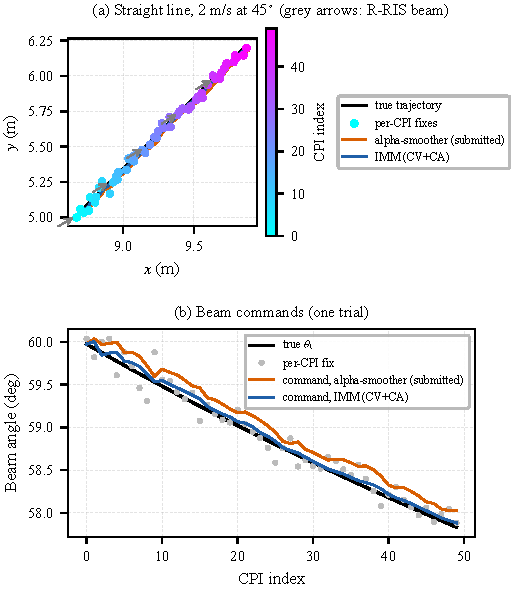
\includegraphics[width=0.9\columnwidth]{F9rev_tracking_cv}
\caption{Beam tracking over 50 CPIs (straight line, 2\,m/s). (a) True trajectory, per-CPI position fixes (colour: CPI index) and the tracks of the $\alpha$-smoother and the IMM; grey arrows show the \Rris{} beam. (b) Beam commands: true bearing, per-CPI fix bearing, and the commands of the $\alpha$-smoother, which lags, and the IMM.}
\label{fig:tracking}
\end{figure}

\subsection{R-RIS Beam Update and Tracking}
\begin{figure}[!t]
\centering
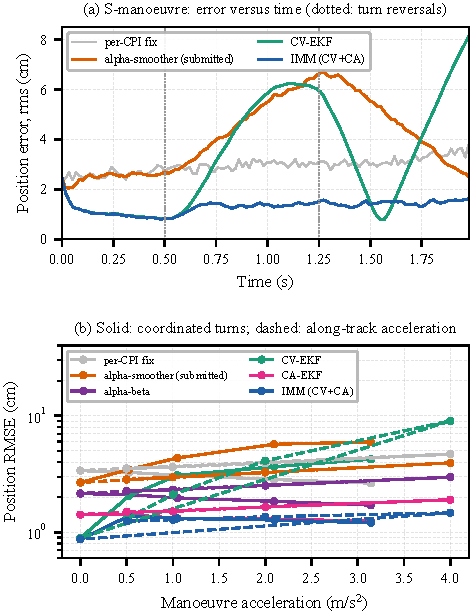
\includegraphics[width=0.9\columnwidth]{FG_tracking_manoeuvre}
\caption{Tracking under manoeuvre (200 Monte Carlo trials). (a) RMS position error versus time through an S-manoeuvre ($\pm60^\circ$/s; dotted: turn reversals). (b) Position RMSE versus manoeuvre acceleration for coordinated turns (solid) and along-track acceleration (dashed).}
\label{fig:manoeuvre}
\end{figure}

\begin{table}[!t]
\centering
\caption{Position RMSE (cm) of the Trackers Under Manoeuvre}
\label{tab:manoeuvre}
\footnotesize
\setlength{\tabcolsep}{1.6pt}
\begin{tabular}{@{}lccccccccc@{}}
\hline\hline
Scenario & $|a|$ & Fix & $\alpha$-sm. & $\alpha$--$\beta$ & CV & CA & IMM & IMM loss \\
 & (m/s$^2$) & & & & & & & max (dB) \\
\hline
Straight line & 0.00 & 3.38 & 2.67 & 2.15 & 0.89 & 1.42 & 0.87 & 0.01 \\
Turn 30$^\circ$/s & 1.05 & 3.08 & 4.34 & 1.97 & 3.08 & 1.32 & 1.31 & 0.01 \\
Turn 90$^\circ$/s & 3.14 & 2.64 & 5.96 & 1.71 & 4.23 & 1.25 & 1.20 & 0.01 \\
Accel. 1 m/s$^2$ & 1.00 & 3.63 & 2.97 & 2.32 & 2.10 & 1.51 & 1.28 & 0.02 \\
Accel. 4 m/s$^2$ & 4.00 & 4.69 & 3.94 & 2.97 & 9.03 & 1.90 & 1.47 & 0.01 \\
S-manoeuvre $\pm$60$^\circ$/s & 2.09 & 2.97 & 4.40 & 1.90 & 3.99 & 1.34 & 1.32 & 0.01 \\
\hline\hline
\multicolumn{9}{@{}p{0.97\columnwidth}@{}}{\scriptsize 2\,s trajectories starting at 2\,m/s; turns from 0.5\,s, acceleration from 0.5 to 1.25\,s; CV/CA/IMM fuse the Doppler path rate. ``IMM loss'': worst-frame illumination loss from pointing error.}
\end{tabular}
\end{table}

Fig.~\ref{fig:tracking} and Table~\ref{tab:tracking} present the straight-line scenario over 50 CPIs (860\,ms): the target moves at 2\,m/s, its bearing from the RIS falls from $60.0^\circ$ to $57.8^\circ$ and its range grows from 10 to 11.7\,m. The per-CPI fixes have an RMSE of 2.76\,cm. The $\alpha$-smoother, which filters the bearing without prediction, reduces this only to 2.56\,cm, and its command visibly lags the true bearing [Fig.~\ref{fig:tracking}(b)]. The IMM, which predicts one CPI ahead and fuses the Doppler path rate, reaches 0.97\,cm (95th percentile 1.87\,cm) and estimates the velocity to 5.3\,cm/s. Pointing is not the limiting factor: with a 12.7$^\circ$ beam, the illumination loss stays below 0.020\,dB for every tracker.

Under manoeuvre the trackers separate (Fig.~\ref{fig:manoeuvre}, Table~\ref{tab:manoeuvre}). In coordinated turns up to $90^\circ$/s (3.1\,m/s$^2$ lateral acceleration) and along-track accelerations up to 4\,m/s$^2$, the CV-EKF lags and its error grows to 9.0\,cm, and the $\alpha$-smoother reaches 6.0\,cm, whereas the IMM stays between 0.87 and 1.47\,cm, within 15\,\% of the best single-model filter in every scenario. The worst-frame illumination loss remains below 0.06\,dB for all trackers, so the beam never loses the target: the choice of tracker governs the accuracy of the reported position and velocity, not the illumination. The measurement model reproduces the signal-level estimator of Section~\ref{sec:efficiency} along the trajectory to within 2\,\% (path) and 1\,\% (path rate), and every frame remains above the $-24$\,dB estimator threshold (lowest -22.2\,dB).

\section{RIS Design Parameters}
\label{sec:design}

\begin{figure*}[!t]
\centering
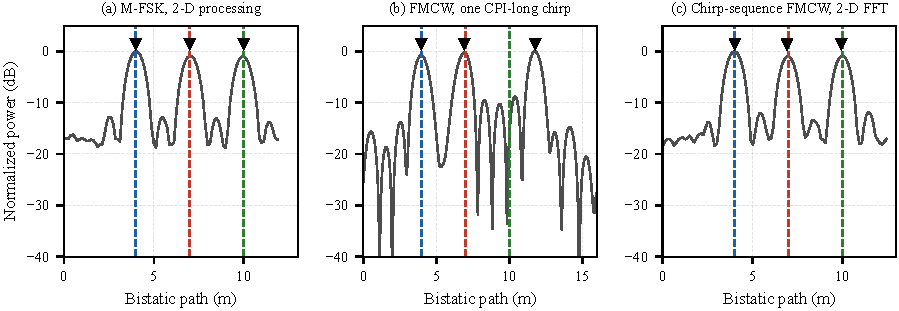
\includegraphics[width=\textwidth]{F11rev_fmcw_fair}
\caption{Three-target scene (bistatic paths 4, 7 and 10\,m; path rates 0, $+3$ and $-2$\,m/s) at equal bandwidth, CPI and energy. (a) M-FSK with 2-D processing. (b) FMCW with one chirp spanning the CPI; range--Doppler coupling moves the two moving targets (arrows). (c) Chirp-sequence FMCW with a 2-D FFT. Dashed: true paths; triangles: detections.}
\label{fig:multitarget}
\end{figure*}

\subsection{Multi-Target Capability and System Power}
\begin{figure*}[!t]
\centering
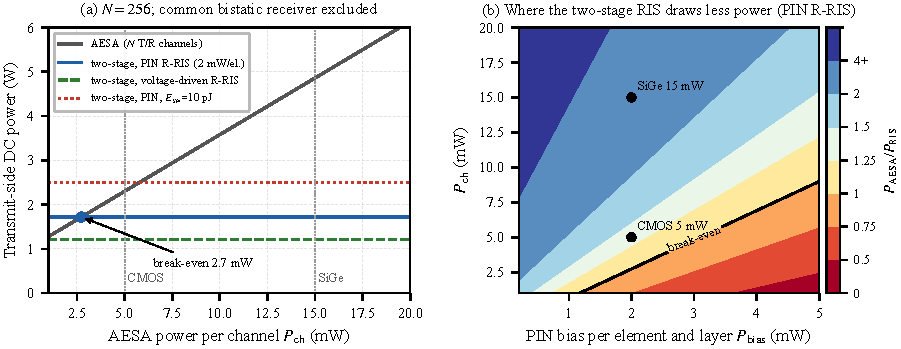
\includegraphics[width=\textwidth]{F12rev_power}
\caption{Transmit-side DC power with the common bistatic receiver excluded. (a) Two-stage RIS (PIN or voltage-driven \Rris{}, and a pessimistic switching energy) versus an AESA as a function of its per-channel power, $N=256$. (b) Ratio of AESA to two-stage power versus PIN bias per element and layer and AESA channel power.}
\label{fig:power}
\end{figure*}

\begin{table*}[!t]
\centering
\caption{Two-Stage Versus Single-Stage Architectures for Steered M-FSK Generation}
\label{tab:arch_comparison}
\footnotesize
\begin{tabular}{@{}lccc@{}}
\hline\hline
 & Two-stage T-RIS/R-RIS & Single stage, per-symbol reload & Single stage, FPGA/LUT or global line \\
\hline
Control writes per symbol & one DDS word & $NB$ bits (SPI) & pointer (LUT) \\
Symbol rate & 714 kHz$^\dagger$ & 13.0 kHz & 2.1 MHz$^\ddagger$ \\
Elements switched at $f_m$ & $N$ (T-RIS only) & $N$ (all) & $N$ (all) \\
Distinct modulation drives & 1 (common) & $N$ & $N$ or 1 global line \\
Drive timing resolution & none & 0.42 ns & 0.42 ns / none \\
Beamformer technology & any (static per CPI) & fast switching & fast switching \\
Beamformer update & 45 kbit/s & per symbol & per symbol / per CPI \\
Inter-stage coupling loss & $C_0^2$ (Sec.~\ref{sec:5b}) & none & none \\
Carrier feedthrough & $|T_{\rm mean}|$ & suppressible & suppressed (0/$\pi$) \\
\hline\hline
\multicolumn{4}{@{}p{0.98\textwidth}@{}}{\scriptsize $N=256$, $B=3$ bits, $f_{m,M}=300$\,MHz, SPI at 10\,MHz. $^\dagger$Set by $T_{\rm sym}=1.4\,\mu$s; the DDS itself switches in tens of ns. $^\ddagger$16 parallel chains at 100\,MHz. Per-element phase offsets imposed by time coding need a timing resolution of $1/(2^B f_{m,M})$; a global 0/$\pi$ line that toggles every element's phase state avoids it but still switches all beamforming elements at $f_m$.}
\end{tabular}
\end{table*}

M-FSK resolves $K$ targets from the linear IFFT of the coherently averaged tone phasors \eqref{eq:ybar}, producing one peak per target without cross-products and resolving up to $M-1$ targets in one Doppler cell~\cite{rohling2001waveform}. Fig.~\ref{fig:multitarget} compares it with FMCW for a three-target scene (bistatic paths 4, 7 and 10\,m; path rates 0, $+3$ and $-2$\,m/s) at equal bandwidth (300\,MHz), CPI and energy. With two-dimensional processing, M-FSK places the three peaks at the true paths [Fig.~\ref{fig:multitarget}(a)]. A single chirp spanning the whole CPI [Fig.~\ref{fig:multitarget}(b)] displaces each moving target by $\dot L f_c T_{\mathrm{CPI}}/B$, i.e., 1.61\,m per m/s, and produces detections at 11.8 and 6.9\,m that coincide with no target; this configuration is not representative of FMCW practice. A sequence of $N_{\mathrm{sw}}$ chirps of duration $T_{\mathrm{sw}}$ processed by a 2-D FFT [Fig.~\ref{fig:multitarget}(c)] reduces the coupling to 1.6\,mm per m/s and resolves the three targets as M-FSK does. At equal CPI the two waveforms therefore achieve the same multi-target resolution. In the proposed architecture M-FSK is preferred for implementation reasons: it needs 3.9 times fewer FFT operations per CPI here, and it is produced by switching one DDS between discrete tones, so that the response of the \Tris{} modulator is calibrated per tone rather than across a continuous sweep.

Table~\ref{tab:arch_comparison} compares the architectures. A single stage can match or exceed the two-stage symbol rate once its phase maps are loaded in parallel, but it must then switch every beamforming element at $f_m$. The two-stage design confines this switching to the \Tris{}, driven by one DDS, and updates the \Rris{} once per CPI (45\,kbit/s), at the cost of the inter-stage coupling loss $C_0^2$.

For power, the bistatic receiver (LNA, ADC and DSP, 0.63\,W) is common to all architectures and is excluded. The transmit side of the two-stage RIS comprises the CW source (0.5\,W at 20\,\% power-amplifier efficiency), the bias of both layers, the \Tris{} switching and the controller,
\begin{equation}
P_{\mathrm{RIS}} = \frac{P_{\mathrm{Tx}}}{\eta} + N\big(P_{\mathrm{b,T}} + P_{\mathrm{b,R}}\big) + 2N\bar f_m E_{\mathrm{sw}} + P_{\mathrm{ctrl}},
\label{eq:Pris_dc}
\end{equation}
where $\bar f_m$ is the mean tone frequency. For a PIN diode the switching energy is set by the stored charge, $E_{\mathrm{sw}} \approx Q_s V \approx P_{\mathrm{b,T}}\tau_{\mathrm{sw}}$, rather than by the junction capacitance ($\tfrac12 C_J V^2 = 9.6$\,fJ); with $\tau_{\mathrm{sw}} = 0.27$\,ns (Section~\ref{sec:sideband}) and $P_{\mathrm{b}} = 2$\,mW per element and layer, $E_{\mathrm{sw}} \approx 0.54$\,pJ. An $N$-element AESA transmitter draws~\cite{kibaroglu2018low,wang2024reconfigurable}
\begin{equation}
P_{\mathrm{AESA}} = N P_{\mathrm{ch}} + P_{\mathrm{LO}} + P_{\mathrm{ctrl}},
\label{eq:Paesa}
\end{equation}
with $P_{\mathrm{LO}} = 0.87$\,W for local-oscillator distribution and the main amplifier. For $N = 256$ [Fig.~\ref{fig:power}(a), Table~S4], the two-stage RIS draws 1.72\,W, 25\,\% less than an AESA with $P_{\mathrm{ch}} = 5$\,mW (2.30\,W), representative of recent CMOS beamformers, and 65\,\% less than with 15\,mW (4.86\,W); the two break even at $P_{\mathrm{ch}} = 2.7$\,mW. Both totals scale linearly with $N$ through the per-element costs $2P_{\mathrm b}$ and $P_{\mathrm{ch}}$, so the comparison does not change with array size. Fig.~\ref{fig:power}(b) maps the ratio: the advantage requires the PIN bias to stay below about half the AESA channel power. A voltage-driven \Rris{} (varactor or liquid crystal), which the two-stage architecture permits because the \Rris{} never switches at the modulation rate, lowers the total to 1.21\,W (48\,\% below the CMOS AESA); a pessimistic $E_{\mathrm{sw}} = 10$\,pJ raises it to 2.51\,W.

\begin{figure}[!t]
\centering
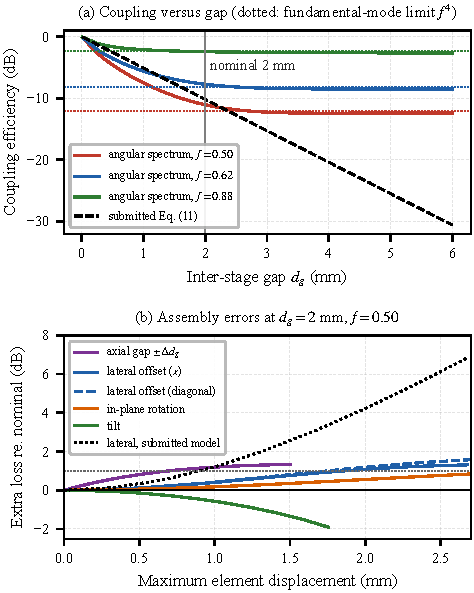
\includegraphics[width=0.9\columnwidth]{FH_interlayer_coupling}
\caption{Inter-stage coupling from the Rayleigh--Sommerfeld (angular-spectrum) model. (a) Coupling efficiency versus gap for element apertures of fill factor $f$, with the on-axis model \eqref{eq:C0}; dotted lines mark the fundamental-mode limit $f^4$. (b) Extra loss versus the maximum element displacement produced by each assembly error at $d_g=2$\,mm and $f=0.5$; negative values are gains.}
\label{fig:gap_sensitivity}
\end{figure}

\subsection{Inter-Stage Coupling and Assembly Tolerance}
\label{sec:5b}
\begin{table}[!t]
\centering
\caption{Hardware and Assembly Tolerance Budget ($d_g=2$\,mm, patch fill $f=0.50$)}
\label{tab:tolerance}
\footnotesize
\setlength{\tabcolsep}{1.3pt}
\begin{tabular}{@{}lcccl@{}}
\hline\hline
Impairment & 0.5\,dB & 1\,dB & Submitted & Note \\
\hline
Phase noise $\sigma_\phi$ & 19\,$^\circ$ & 27\,$^\circ$ & -- & beyond 3-bit \\
Switching jitter $\sigma_t$ & 180\,ps & 255\,ps & -- & at 300\,MHz \\
Osc. linewidth $\Delta\nu$ & 6.6\,Hz & 13.6\,Hz & -- & $v$: $\times$1.9 at 0.3\,Hz \\
Axial gap $|\Delta d_g|$ & 0.27\,mm & 0.70\,mm & 0.10\,/\,0.20\,mm &  \\
Lateral, $x$ & 1.13\,mm & 1.86\,mm & 0.62\,/\,0.90\,mm &  \\
Lateral, diagonal & 1.11\,mm & 1.75\,mm & -- &  \\
Rotation & 1.86\,mm & $>$3.0\,mm & -- & 3$^\circ$ = 3.0\,mm \\
Tilt & none & none & -- & gain; $\le$0.33$^\circ$ pointing \\
\hline\hline
\multicolumn{5}{@{}p{0.97\columnwidth}@{}}{\scriptsize Tolerances give the impairment that costs 0.5 or 1\,dB of array gain (phase noise, assembly) or of coherent-integration gain (linewidth). Assembly values are maximum element displacements from the angular-spectrum model; ``Submitted'' is the on-axis exponential model \eqref{eq:C0}. A 1\,dB loss raises the position RMSE by 12\,\%, the estimator remaining efficient.}
\end{tabular}
\end{table}

The received power is proportional to the inter-stage coupling efficiency, $C_0^2$ in \eqref{eq:Prx}. To quantify assembly errors, the on-axis approximation \eqref{eq:C0} is replaced by the scalar Rayleigh--Sommerfeld model it approximates, evaluated by angular-spectrum propagation of the finite $16\times16$ \Tris{} aperture field to the \Rris{} plane. Each element is represented by a square aperture of side $f d$, and the coupled field is averaged over the corresponding \Rris{} aperture; evanescent components decay and the fundamental Floquet mode propagates. Fig.~\ref{fig:gap_sensitivity}(a) compares the two models. The full model is continuous with unit coupling as $d_g \to 0$ and saturates at the fundamental-mode limit $f^4$ once the higher-order Floquet harmonics, decaying at $\sqrt{3}\,(2\pi/\lambda)$, have died out. For $f = 0.5$ it gives $-11.1$\,dB at the 2\,mm nominal gap, within 0.9\,dB of \eqref{eq:C0}, and a local slope of 2.2\,dB/mm rather than 5.1\,dB/mm.

Fig.~\ref{fig:gap_sensitivity}(b) and Table~\ref{tab:tolerance} report the extra loss caused by assembly errors at $d_g = 2$\,mm with $f = 0.5$, the most sensitive of the fill factors considered. A 1-dB loss requires a gap increase of 0.70\,mm (the on-axis model gave 0.20\,mm), a lateral offset of 1.86\,mm ($0.35\,d$) along a lattice axis or 1.75\,mm diagonally, and more than $3^\circ$ of in-plane rotation (0.94\,dB at $3^\circ$). Tilting the \Tris{} brings half of the aperture closer to the \Rris{} and increases the coupling up to physical contact at $2.6^\circ$, while biasing the beam by at most $0.33^\circ$. Because the estimator remains efficient (Section~\ref{sec:efficiency}), a 1-dB loss raises the position RMSE by 12\,\%. These tolerances lie within standard mmWave PCB assembly practice. The scalar model captures propagation and evanescent decay between the apertures, but not the loading of the diode circuits by the near field of the other layer, which requires full-wave simulation of the stacked unit cell.

\begin{figure}[!t]
\centering
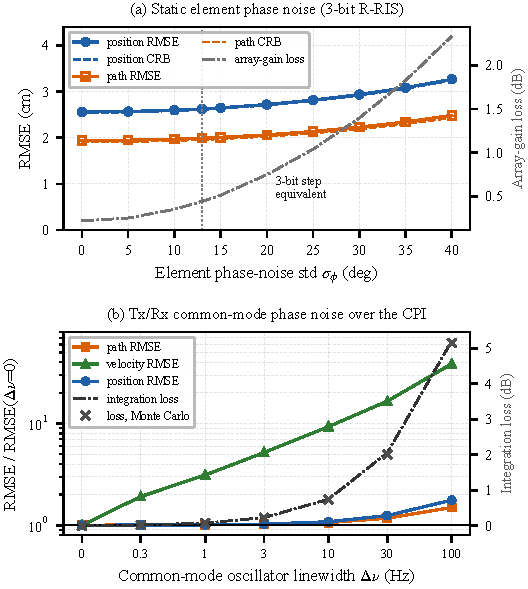
\includegraphics[width=0.9\columnwidth]{FF_phase_noise}
\caption{(a) Path and position RMSE (Monte Carlo) and bounds versus the element phase-noise standard deviation, on top of 3-bit quantization, with the resulting array-gain loss. (b) RMSE relative to a noiseless oscillator versus the common-mode Tx/Rx linewidth, with the coherent-integration loss (closed form and Monte Carlo).}
\label{fig:phase_noise}
\end{figure}

\subsection{Element Phase Noise and Oscillator Coherence}
\label{sec:phase_noise}
Static element phase errors arise from fabrication and bias spread of the \Tris{} sideband and \Rris{} reflection phases. Modelling them as independent Gaussian errors of standard deviation $\sigma_\phi$ added to the 3-bit phases, Fig.~\ref{fig:phase_noise}(a) shows that the array-gain loss follows $e^{-\sigma_\phi^2}$ to within 0.01\,dB and that the Monte Carlo path and position RMSE remain on their bounds throughout, the RMSE-to-CRB ratio changing by less than 1\,\%. The 3-bit quantization itself costs 0.22\,dB, equivalent to $\sigma_\phi = 13^\circ$. An additional $\sigma_\phi$ of $19^\circ$ costs 0.5\,dB and $27^\circ$ costs 1\,dB; at $20^\circ$ the position RMSE rises from 2.56 to 2.72\,cm (6\,\%). Random phase noise adds only $0.14^\circ$ rms of pointing error at $\sigma_\phi = 20^\circ$.

Dynamic phase noise has two sources. Jitter $\sigma_t$ in the switching instants of the PIN diodes, independent across elements and symbols, reduces the sideband power by $e^{-(2\pi f_{m,k}\sigma_t)^2}$; at 300\,MHz this reaches 0.5\,dB only for $\sigma_t = 180$\,ps. The common-mode phase noise of the Tx CW source and the Rx local oscillator is more demanding in a bistatic link, where the two are physically separate. Modelled as a Wiener process of linewidth $\Delta\nu$, it reduces the coherent-integration gain by $\eta = 2(x-1+e^{-x})/x^2$ with $x = \pi\Delta\nu T_{\mathrm{CPI}}$, which agrees with Monte Carlo to within 0.1\,dB [Fig.~\ref{fig:phase_noise}(b)]; the loss reaches 0.5\,dB at $\Delta\nu = 6.6$\,Hz. Path and position RMSE rise by 6\,\% and 8\,\% at 10\,Hz, but the velocity estimate, whose bound corresponds to about 1\,Hz of Doppler, is 1.9 times worse already at 0.3\,Hz. The Tx and Rx must therefore be locked to a common frequency reference, as is standard in coherent bistatic radar.

\begin{figure}[!t]
\centering
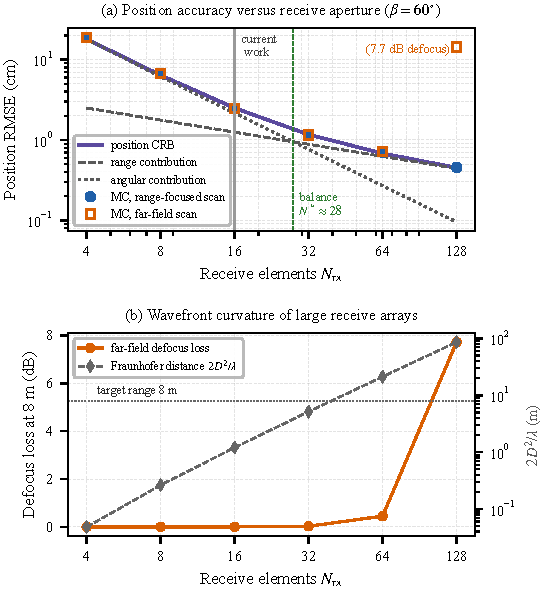
\includegraphics[width=0.9\columnwidth]{FI_rx_aperture}
\caption{(a) Position RMSE (Monte Carlo) and bound versus the number of receive elements, with the range and angular contributions to the bound; far-field and range-focused beam scanning. (b) Wavefront-curvature (defocus) loss of far-field scanning at the Rx--target range, and the Fraunhofer distance of the array.}
\label{fig:aperture}
\end{figure}

\subsection{Receive Aperture Scaling}
\label{sec:aperture}
Because angular estimation dominates the position error at $N_{\mathrm{rx}} = 16$, Fig.~\ref{fig:aperture}(a) and Table~S3 vary the receive array from 4 to 128 half-wavelength elements. Both contributions improve: the array gain raises $\mathrm{SNR}_1$ by $10\log_{10}(N_{\mathrm{rx}}/16)$, so the path error falls as $N_{\mathrm{rx}}^{-1/2}$, while the angle bound \eqref{eq:crb_theta} falls as $N_{\mathrm{rx}}^{-3/2}$ (Monte Carlo slopes -0.49 and -1.50). The range and angular contributions to \eqref{eq:crb_pos} balance at $N^* \approx 28$ elements. Doubling the array to 32 elements halves the position RMSE, from 2.46 to 1.15\,cm, and 64 elements reduce it 3.5-fold to 0.70\,cm, beyond which the path error dominates and returns diminish.

Large arrays are, however, inside their Fraunhofer distance $2D^2/\lambda$ at the 8\,m Rx--target range [Fig.~\ref{fig:aperture}(b)]. Far-field beam scanning loses 0.45\,dB to wavefront curvature at 64 elements and 7.7\,dB at 128, where it fails (14.3\,cm). Focusing the scan at the Rx--target distance, which the path estimate already provides, restores the bound (0.45\,cm) at every size.

\section{Conclusion}
\label{sec:conclusion}
This paper presented a two-stage PIN-diode RIS for M-FSK sensing at 28\,GHz in which a \Tris{}, driven by a single DDS, generates the tones and an \Rris{}, updated once per CPI, steers them. Separating the functions confines radio-frequency switching to one layer, whereas a single surface that both modulates and beamforms must switch every beamforming element at the modulation rate. The tones are separated in a complex-baseband receiver, where quadrature imbalance produces only a Doppler-mirror ghost 36.8\,dB below the target, and their squint costs 0.03\,dB while $N_xB_f\sin\theta_1 \lesssim 0.5$.

A coherent two-dimensional estimator with peak refinement attains the path, velocity and angle bounds (1.84\,cm, 0.59\,cm/s and $0.134^\circ$), and the bistatic position RMSE of 2.45\,cm matches its Jacobian bound at a $60^\circ$ bistatic angle; phase quantization, element spread, phase noise and pointing error reduce the SNR without degrading estimator efficiency. An IMM tracker with Doppler fusion keeps the position RMSE between 0.87 and 1.47\,cm under turns up to $90^\circ$/s and accelerations up to 4\,m/s$^2$. A Rayleigh--Sommerfeld analysis of the inter-stage coupling gives assembly tolerances of 0.70\,mm in gap and 1.86\,mm laterally, and velocity estimation requires the Tx and Rx to share a frequency reference. With identical accounting the transmit side draws 25\,\% less power than a 5-mW-per-channel CMOS AESA, and at equal CPI the waveform matches chirp-sequence FMCW in multi-target resolution.

Future work will validate the stacked unit cell by full-wave simulation and measurement, rebuild the link budget from the validated coupling, study dense multi-target scenes, and use larger receive arrays with range-focused processing, which would reduce the position error 2.1-fold with 32 elements and 3.5-fold with 64. Code for the simulations and analyses is provided in the \href{https://github.com/PavanMohanN/2S_RIS_MFSK}{GitHub Repository}.

\begin{thebibliography}{10}
\bibitem{wu2019towards}
Q.~Wu and R.~Zhang, ``Towards smart and reconfigurable environment: Intelligent reflecting surface aided wireless network,'' \emph{IEEE Commun. Mag.}, vol.~58, no.~1, pp.~106--112, Jan. 2020.

\bibitem{basar2019wireless}
E.~Basar, M.~Di~Renzo, J.~De~Rosny, M.~Debbah, M.-S. Alouini, and R.~Zhang, ``Wireless communications through reconfigurable intelligent surfaces,'' \emph{IEEE Access}, vol.~7, pp.~116\,753--116\,773, 2019.

\bibitem{hu2018beyond}
S.~Hu, F.~Rusek, and O.~Edfors, ``Beyond massive MIMO: The potential of data transmission with large intelligent surfaces,'' \emph{IEEE Trans. Signal Process.}, vol.~66, no.~10, pp.~2746--2758, May 2018.

\bibitem{marzetta2015massive}
T.~L. Marzetta, ``Massive MIMO: An introduction,'' \emph{Bell Labs Tech. J.}, vol.~20, pp.~11--22, 2015.

\bibitem{liaskos2018new}
C.~Liaskos, S.~Nie, A.~Tsioliaridou, A.~Pitsillides, S.~Ioannidis, and I.~Akyildiz, ``A new wireless communication paradigm through software-controlled metasurfaces,'' \emph{IEEE Commun. Mag.}, vol.~56, no.~9, pp.~162--169, Sep. 2018.

\bibitem{wu2019intelligent}
Q.~Wu and R.~Zhang, ``Intelligent reflecting surface enhanced wireless network via joint active and passive beamforming,'' \emph{IEEE Trans. Wireless Commun.}, vol.~18, no.~11, pp.~5394--5409, Nov. 2019.

\bibitem{zhang2018space}
L.~Zhang \emph{et al.}, ``Space-time-coding digital metasurfaces,'' \emph{Nature Commun.}, vol.~9, no.~1, Art. no.~4334, 2018.

\bibitem{rohling2001waveform}
H.~Rohling and M.-M. Meinecke, ``Waveform design principles for automotive radar systems,'' in \emph{Proc. CIE Int. Conf. Radar}, Beijing, China, 2001, pp.~1--4.

\bibitem{lu2024integrated}
S.~Lu \emph{et al.}, ``Integrated sensing and communications: Recent advances and ten open challenges,'' \emph{IEEE Internet Things J.}, vol.~11, no.~11, pp.~19\,094--19\,120, Jun. 2024.

\bibitem{zhang2019breaking}
L.~Zhang \emph{et al.}, ``Breaking reciprocity with space-time-coding digital metasurfaces,'' \emph{Adv. Mater.}, vol.~31, no.~41, Art. no.~1904069, 2019.

\bibitem{dai2018independent}
J.~Y. Dai, J.~Zhao, Q.~Cheng, and T.~J. Cui, ``Independent control of harmonic amplitudes and phases via a time-domain digital coding metasurface,'' \emph{Light Sci. Appl.}, vol.~7, no.~1, Art. no.~90, 2018.

\bibitem{shen2025sub}
D.~Shen \emph{et al.}, ``Sub-terahertz transmissive reconfigurable intelligent surface for integrated beam steering and self-OOK-modulation,'' \emph{Light Sci. Appl.}, vol.~14, no.~1, Art. no.~13, 2025.

\bibitem{zhao2019programmable}
J.~Zhao \emph{et al.}, ``Programmable time-domain digital-coding metasurface for non-linear harmonic manipulation and new wireless communication systems,'' \emph{Nat. Sci. Rev.}, vol.~6, no.~2, pp.~231--238, 2019.

\bibitem{liaskos2022software}
C.~Liaskos \emph{et al.}, ``Software-defined reconfigurable intelligent surfaces: From theory to end-to-end implementation,'' \emph{Proc. IEEE}, vol.~110, no.~9, pp.~1466--1493, Sep. 2022.

\bibitem{demmer2023hybrid}
D.~Demmer \emph{et al.}, ``Hybrid precoding applied to multi-beam transmitting reconfigurable intelligent surfaces (T-RIS),'' \emph{Electronics}, vol.~12, no.~5, Art. no.~1162, 2023.

\bibitem{dai2020reconfigurable}
L.~Dai \emph{et al.}, ``Reconfigurable intelligent surface-based wireless communications: Antenna design, prototyping, and experimental results,'' \emph{IEEE Access}, vol.~8, pp.~45\,913--45\,923, 2020.

\bibitem{pozar2011microwave}
D.~M. Pozar, \emph{Microwave Engineering}, 4th~ed. Hoboken, NJ, USA: Wiley, 2011.

\bibitem{song2018beam}
Q.~Song, Y.~Wang, K.~Liu, J.~Zhang, and Y.~Wang, ``Beam steering for OAM beams using time-modulated circular arrays,'' \emph{Electron. Lett.}, vol.~54, no.~17, pp.~1017--1018, 2018.

\bibitem{marcuvitz1951waveguide}
N.~Marcuvitz, \emph{Waveguide Handbook} (IEE Electromagnetic Waves Series 21). London, U.K.: Peter Peregrinus, 1986, reprint of the 1951 ed., MIT Radiation Laboratory Series, vol.~10.

\bibitem{pfeiffer2013cascaded}
C.~Pfeiffer and A.~Grbic, ``Cascaded metasurfaces for complete phase and polarization control,'' \emph{Appl. Phys. Lett.}, vol.~102, no.~23, Art. no.~231116, 2013.

\bibitem{monticone2017metamaterial}
F.~Monticone and A.~Al\`u, ``Metamaterial, plasmonic and nanophotonic devices,'' \emph{Rep. Prog. Phys.}, vol.~80, no.~3, Art. no.~036401, 2017.

\bibitem{an2025stacked}
J.~An, M.~Di~Renzo, M.~Debbah, H.~V. Poor, and C.~Yuen, ``Stacked intelligent metasurfaces for multiuser downlink beamforming in the wave domain,'' \emph{IEEE Trans. Wireless Commun.}, 2025.

\bibitem{balanis2016antenna}
C.~A. Balanis, \emph{Antenna Theory: Analysis and Design}, 4th~ed. Hoboken, NJ, USA: Wiley, 2016.

\bibitem{mailloux2017phased}
R.~J. Mailloux, \emph{Phased Array Antenna Handbook}, 3rd~ed. Norwood, MA, USA: Artech House, 2017.

\bibitem{willis2005bistatic}
N.~J. Willis, \emph{Bistatic Radar}, 2nd~ed. Raleigh, NC, USA: SciTech, 2005.

\bibitem{tang2020wireless}
W.~Tang \emph{et al.}, ``Wireless communications with reconfigurable intelligent surface: Path loss modeling and experimental measurement,'' \emph{IEEE Trans. Wireless Commun.}, vol.~20, no.~1, pp.~421--439, Jan. 2021.

\bibitem{van2002optimum}
H.~L. Van~Trees, \emph{Optimum Array Processing: Part IV of Detection, Estimation, and Modulation Theory}. New York, NY, USA: Wiley, 2002.

\bibitem{krim2002two}
H.~Krim and M.~Viberg, ``Two decades of array signal processing research: The parametric approach,'' \emph{IEEE Signal Process. Mag.}, vol.~13, no.~4, pp.~67--94, Jul. 1996.

\bibitem{steven1993fundamentals}
S.~M. Kay, \emph{Fundamentals of Statistical Signal Processing: Estimation Theory}. Englewood Cliffs, NJ, USA: Prentice-Hall, 1993.

\bibitem{richards2005fundamentals}
M.~A. Richards, \emph{Fundamentals of Radar Signal Processing}. New York, NY, USA: McGraw-Hill, 2005.

\bibitem{harris1978use}
F.~J. Harris, ``On the use of windows for harmonic analysis with the discrete Fourier transform,'' \emph{Proc. IEEE}, vol.~66, no.~1, pp.~51--83, Jan. 1978.

\bibitem{willis2007advances}
N.~J. Willis and H.~D. Griffiths, Eds., \emph{Advances in Bistatic Radar}. Raleigh, NC, USA: SciTech, 2007.

\bibitem{bar2001estimation}
Y.~Bar-Shalom, X.~R. Li, and T.~Kirubarajan, \emph{Estimation with Applications to Tracking and Navigation: Theory, Algorithms and Software}. New York, NY, USA: Wiley, 2001.

\bibitem{blackman1999design}
S.~S. Blackman and R.~Popoli, \emph{Design and Analysis of Modern Tracking Systems}. Norwood, MA, USA: Artech House, 1999.

\bibitem{hillerdesign}
G.~Hiller, ``Design with PIN diodes,'' M/A-COM, Lowell, MA, USA, Appl. Note AG312, 1998. [Online]. Available: \url{https://cdn.macom.com/applicationnotes/AG312.pdf}

\bibitem{kibaroglu2018low}
K.~Kibaroglu, M.~Sayginer, and G.~M. Rebeiz, ``A low-cost scalable 32-element 28-GHz phased array transceiver for 5G communication links based on a $2\times2$ beamformer flip-chip unit cell,'' \emph{IEEE J. Solid-State Circuits}, vol.~53, no.~5, pp.~1260--1274, May 2018.

\bibitem{wang2024reconfigurable}
J.~Wang \emph{et al.}, ``Reconfigurable intelligent surface: Power consumption modeling and practical measurement validation,'' \emph{IEEE Trans. Commun.}, vol.~72, no.~9, pp.~5720--5734, Sep. 2024.
\end{thebibliography}

\end{document}
